%% abtex2-modelo-artigo.tex, v-1.9.7 laurocesar
%% Copyright 2012-2018 by abnTeX2 group at http://www.abntex.net.br/ 
%%
%% This work may be distributed and/or modified under the
%% conditions of the LaTeX Project Public License, either version 1.3
%% of this license or (at your option) any later version.
%% The latest version of this license is in
%%   http://www.latex-project.org/lppl.txt
%% and version 1.3 or later is part of all distributions of LaTeX
%% version 2005/12/01 or later.
%%
%% This work has the LPPL maintenance status `maintained'.
%% 
%% The Current Maintainer of this work is the abnTeX2 team, led
%% by Lauro César Araujo. Further information are available on 
%% http://www.abntex.net.br/
%%
% ------------------------------------------------------------------------
% ------------------------------------------------------------------------
% abnTeX2: Modelo de Artigo Acadêmico em conformidade com
% ABNT NBR 6022:2018: Informação e documentação - Artigo em publicação 
% periódica científica - Apresentação
% ------------------------------------------------------------------------
% ------------------------------------------------------------------------

\documentclass[
	% -- opções da classe memoir --
	article,			% indica que é um artigo acadêmico
	12pt,				% tamanho da fonte
	oneside,			% para impressão apenas no recto. Oposto a twoside
	a4paper,			% tamanho do papel. 
	% -- opções da classe abntex2 --
	%chapter=TITLE,		% títulos de capítulos convertidos em letras maiúsculas
	%section=TITLE,		% títulos de seções convertidos em letras maiúsculas
	%subsection=TITLE,	% títulos de subseções convertidos em letras maiúsculas
	%subsubsection=TITLE % títulos de subsubseções convertidos em letras maiúsculas
	% -- opções do pacote babel --
    BIBLATEX,           % indica para utilizar BIBLATEX em vez do abntex2cite
	english,			% idioma adicional para hifenização
	brazil,				% o último idioma é o principal do documento
	sumario=tradicional
	]{abntex2}


% ---
% PACOTES
% ---

% ---
% Pacotes fundamentais 
% ---
\usepackage{sbc-template}
\usepackage{times}			% Usa a fonte Times new Roman
\usepackage[T1]{fontenc}		% Selecao de codigos de fonte.
\usepackage[utf8]{inputenc}		% Codificacao do documento (conversão automática dos acentos)
\usepackage{indentfirst}		% Indenta o primeiro parágrafo de cada seção.
\usepackage{nomencl} 			% Lista de simbolos
\usepackage{color}				% Controle das cores
\usepackage{graphicx}			% Inclusão de gráficos
\usepackage{microtype} 			% para melhorias de justificação
\usepackage{tikz}               % para ticks
\usepackage{longtable}          % para quebra de tabela por página
\usepackage{tabularray}         % formatação da coluna e linha da tabela
\usepackage{graphicx}           % utilizado para formatação de tabelas
\usepackage{subcaption}         % para subFiguras
% ---
		
% ---
% Pacotes adicionais, usados apenas no âmbito do Modelo Canônico do abnteX2
% ---
\usepackage{lipsum}				% para geração de dummy text
% ---
		
% ---
% Pacotes de citações
% ---
\usepackage[brazilian,hyperpageref]{backref}	 % Paginas com as citações na bibl
\usepackage[alf]{abntex2cite}	% Citações padrão ABNT
% ---

% Pacotes instalados por nós alunos
\usepackage{xurl}

% ---
% Configurações do pacote backref
% Usado sem a opção hyperpageref de backref
\renewcommand{\backrefpagesname}{Citado na(s) página(s):~}
% Texto padrão antes do número das páginas
\renewcommand{\backref}{}
% Define os textos da citação
\renewcommand*{\backrefalt}[4]{
	\ifcase #1 %
		Nenhuma citação no texto.%
	\or
		Citado na página #2.%
	\else
		%Citado #1 vezes nas páginas #2.%
        Citado nas páginas #2.%
	\fi}%
% ---

% --- Informações de dados para CAPA e FOLHA DE ROSTO ---

\newcommand\nomeprojeto{MyMed}

\def\checkmark{\tikz\fill[scale=0.4](0,.35) -- (.25,0) -- (1,.7) -- (.25,.15) -- cycle;} 

\title{\nomeprojeto}

\author{
Arthur Augusto Lessa Ferreira\inst{1}\thanks{thurlessaf@gmail.com}, 
Fernando Freitas de Lira\inst{1}\thanks{freitaslira18@gmail.com},
\\ Henriquy Dias Terto Alves\inst{1}\thanks{henriquydta@gmail.com},
Isabella Pantolfo Melo\inst{1}\thanks{isabellapantolfo1101@gmail.com}, 
\\ Lucas da Conceição Silva Moura\inst{1}\thanks{pf.lucasmoura@gmail.com},
Mateus Armando Carrara de Mendonça\inst{1}\thanks{mateusacdem@gmail.com }}


\address{
    Instituto Federal de Educação, Ciência e Tecnologia de São Paulo - Campus\\ São Paulo (IFSP) - Rua Pedro Vicente, 625 - Bloco C
}


% ---

% ---
% Configurações de aparência do PDF final

% alterando o aspecto da cor azul
\definecolor{blue}{RGB}{41,5,195}

% informações do PDF
\makeatletter
\hypersetup{
     	%pagebackref=true,
		pdftitle={\@title}, 
		pdfauthor={\@author},
    	pdfsubject={Modelo de artigo científico com abnTeX2},
	    pdfcreator={LaTeX with abnTeX2},
		pdfkeywords={abnt}{latex}{abntex}{abntex2}{atigo científico}, 
		colorlinks=true,       		% false: boxed links; true: colored links
    	linkcolor=blue,          	% color of internal links
    	citecolor=blue,        		% color of links to bibliography
    	filecolor=magenta,      		% color of file links
		urlcolor=blue,
		bookmarksdepth=4
}
\makeatother
% --- 

% ---
% compila o indice
% ---
\makeindex
% ---

% ---
% Altera as margens padrões
% ---
\setlrmarginsandblock{3cm}{3cm}{*} %{ESQUERDA}{DIREITA}
\setulmarginsandblock{3.5cm}{2.5cm}{*} %{SUPERIOR}{INFERIOR}
\checkandfixthelayout
% ---

% --- 
% Espaçamentos entre linhas e parágrafos 
% --- 

% O tamanho do parágrafo é dado por (está definido dentro do sbc-template.sty):
%\setlength{\parindent}{1.3cm}

% Controle do espaçamento entre um parágrafo e outro (está definido dentro do sbc-template.sty):
%\setlength{\parskip}{0.2cm}  % tente também \onelineskip

% Espaçamento simples
% \SingleSpacing


% ----
% Início do             
% ----
\begin{document}

% Seleciona o idioma do documento (conforme pacotes do babel)
%\selectlanguage{english}
\selectlanguage{brazil}


% Retira espaço extra obsoleto entre as frases.
\frenchspacing 

% ----------------------------------------------------------
% ELEMENTOS PRÉ-TEXTUAIS
% ----------------------------------------------------------

%---
%
% Se desejar escrever o artigo em duas colunas, descomente a linha abaixo
% e a linha com o texto ``FIM DE ARTIGO EM DUAS COLUNAS''.
% \twocolumn[    		% INICIO DE ARTIGO EM DUAS COLUNAS
%
%---

% página de titulo principal (obrigatório)
\maketitle

% titulo em outro idioma (opcional)

\begin{abstract}
    This document describes the current architecture of the software designated as ``\nomeprojeto``, which aims to help people maintain their medication supply; and for caregivers maintain medication supplies for all their dependents. In addition, it will offer a scheduling service so that the user can track appointments and blood glucose and blood pressure levels. The content of this document discusses its concept and application, in addition to the data modeling and tools used.
\end{abstract}
     
\begin{resumo1} 
  Este documento descreve a arquitetura presente do software designado como ``\nomeprojeto``, ele visa auxiliar pessoas a manter seu estoque de medicamentos, e para cuidadores manter estoque de medicamentos de todos seus dependentes. Além disso, oferecerá um serviço de agenda para que o usuário acompanhe consultas e taxas de glicemia e pressão. O conteúdo deste documento discorre sobre seu conceito e aplicação, além da modelagem de dados e ferramentas utilizadas.
\end{resumo1}



% ]  				% FIM DE ARTIGO EM DUAS COLUNAS
% ---

%\begin{center}\smaller
%\textbf{Data de submissão e aprovação}: elemento obrigatório. Indicar dia, mês e ano

%\textbf{Identificação e disponibilidade}: elemento opcional. Pode ser indicado o endereço eletrônico, DOI, suportes e outras informações relativas ao acesso.
%\end{center}

% ----------------------------------------------------------
% ELEMENTOS TEXTUAIS
% ----------------------------------------------------------
\textual

% ----------------------------------------------------------
% Introdução
% ----------------------------------------------------------
\section{Introdução}

A saúde dos dias de hoje é em sua maioria amparada, e muitas vezes serve de motivação para serviços tecnológicos como aplicações \textit{mobile}, \textit{sites} de compra de medicamento, informativos \textit{online} de programas do governo, entre outros. Estudos mostram que esses serviços estão em constante evolução e a cada ano sendo mais acessíveis e utilizados por ambos os grupos de médicos e de pacientes \cite{clarisse2016}.

Um grupo muito beneficiado por essas tecnologias é o da terceira idade (idosos com mais de 60 anos). Segundo \citeonline{clarisse2016}, com a idade avançada e capacidades motoras reduzidas, idosos necessitam de aplicativos com interfaces simples e funcionalidades diretas para realizar tarefas do dia a dia ou até dentro do seu celular.

Aplicativos de assistência ao idoso são exemplos de um mercado promissor e possuem uma gama de usuários que buscam estes serviços. Porém, muitas vezes não possuem autonomia própria e não conseguem usar tais sistemas.

Um caso relevante é o de idosos que não possuem autonomia própria e são zelados por cuidadores contratados pela família. Para \citeonline{aline2012sobrecarga}, os profissionais - que são em grande parte mulheres adultas - sofrem de doenças como hipertensão e estresse devido o acúmulo de múltiplos papéis.

\begin{citacao}
"Pode-se verificar relação entre características dos cuidadores com a sobrecarga, em que os cuidadores, na maioria, familiares do sexo feminino, encontram-se na faixa etária adulta, fase em que a mulher tem vários papéis sociais: mãe, esposa, dona de casa, dentre outros. Muitas vezes, tem outras atribuições sociais, como o trabalho fora do lar, além de assumir o cuidado de seus pais, já idosos." \cite{aline2012sobrecarga} 
\end{citacao}

Esses profissionais enfrentam uma rotina intensa, marcada por altos níveis de estresse e responsabilidades, gerando assim problemas de saúde como hipertensão e estresse persistente.

Em vista de todas as oportunidades de mercado para estas soluções, ainda não há uma plataforma que seja clara e direta em sua execução, segundo \citeonline{janaina2023}. Um exemplo é o Sistema Móvel de Assistência ao Idoso (SMAI), que, embora disponibilize suporte para cuidadores de idosos com demência, apresenta limitações significativas, tal qual uma interface repetitiva e a necessidade de preencher fichas técnicas extensas, fato que compromete a usabilidade e a praticidade que esses profissionais necessitam no dia a dia \cite{andre2020}.

Visando superar essas limitações, o projeto propõe o desenvolvimento de uma plataforma focada exclusivamente no cuidador de idosos, com funcionalidades que centralizam o monitoramento e a gestão de tratramentos. A ferramenta inclui lembretes para administração dos remédios, agendamentos de consultadas com calendário integrado, indicação de locais para compra, pesquisa de preços e criação de relatórios médicos - tudo focado na interface intuitiva e direta. Assim, busca-se reduzir a sobrecarga dos cuidadores, proporcionando mais autonamia e eficiência no desempenho de suas funções.
\subsection{Objetivos}

Para o desenvolvimento do sistema, será adotado como referência uma diretriz de desenvolvimento que se baseará na comunicação constante com o usuário e controle das informações.

\subsubsection{Objetivo Geral}

Desenvolver uma plataforma que auxilie os cuidadores de idosos a manter de forma simples, organizada e eficaz o acompanhamento de pacientes. O sistema irá permitir registro de medicamentos utilizados, consultas agendadas e realizadas, com possibilidade de gerar relatórios e gráficos personalizados de acordo com os tratamentos em andamento (como controle de glicemia e hipertensão).

Além disso, enviará alertas sobre o estoque de medicamentos de todos os pacientes vinculados a uma conta, indicando a estimativa de tempo de consumo restante e realizando pesquisas de preços para reposição. 

 Também contará com um módulo de registros de dados médicos, onde o cuidador poderá inserir informações essenciais, como índices de glicemia e pressão arterial, datas de retorno, novas prescrições e informações relevantes para aquele tratamento. 

\subsubsection{Objetivos Específicos}

A fim de alcançar o objetivo geral da proposta apresentada, foram delineados os seguintes objetivos específicos:

\begin{enumerate}
    \item Conduzir entrevistas com cuidadores registrados e funcionários de casas de repouso. Analisar resultados para direcionar a um desenvolvimento próximo ao usuário final da aplicação.
    \item Realizar uma pesquisa de mercado de aplicações similares, a fim de criar uma solução única ao usuário voltada ao melhoramento de recursos já existentes e implantação de recomendações destes usuários. 
    \item Desenvolver um sistema que, com uma interface simples e intuitiva, além de lembretes que auxilie o usuário a manter seu tratamento, automatize uma tarefa banal.
    \item Aplicar as funcionalidades do sistema de forma empírica em um público-alvo a fim de aprimorar o sistema e torná-lo útil ao usuário final.
\end{enumerate}


\subsection{Justificativa}    

Segundo \citeonline{mariacristina2008}, o consumo de um medicamento ou o acompanhamento de consultas de rotina podem se tornar algo supérfluo na rotina de um paciente que os realiza com frequência, podendo acarretar em um esquecimento de tais compromissos. 

A partir disso, foi realizada uma pesquisa com o público geral no formato de um formulário online. Foi apontado que 70\% dos participantes utilizam pouco ou muito pouco de serviços tecnológicos de saúde; dos que utilizam, 63\% relatam não corresponder às suas expectativas. Cerca de 62\% dos participantes têm grandes dificuldades em lembrar de datas de consultas, e 81\% relatam problemas no horário de consumo de remédios.

O \textit{feedback} constante de usuários de sistemas existentes será a base do desenvolvimento, e trará uma solução prática ao público-alvo que aperfeiçoe as aplicações já utilizadas.

Este documento, portanto, demonstra a necessidade de tal sistema. Destinado a usuários que necessitam de um melhor gerenciamento de seus tratamentos, sejam eles medicamentos ou consultas; a fim de manter sua saúde bem condicionada e supervisionada.

\section{Referencial Teórico}

A revisão bibliográfica será dividida em análise do mercado de telemedicina e sua recepção, plataformas de telemonitoramento, e por fim a lacuna no mercado de ferramentas para cuidadores de idosos.

\subsection{Mercado de Telemedicina}

Para \citeonline{janaina2023}, há um crescente número de profissionais da saúde utilizando tecnologias novas para o gerenciamento de seus tratamentos. Estas tecnologias são categorizadas como de `telessaúde`. Dentre as áreas mais comuns tem-se a teleducação (vídeos de manuais a respeito de ferramentas/recursos do serviço de saúde pública) e a tele-consulta (consultas online que tiveram mais popularidade com a população idosa). O autor ressalta que essas tecnologias ainda não são amplamente utilizadas pelo público geral por fatores como dificuldade de acesso e falta de infraestrutura; mas demonstra que o número de pessoas desse grupo diminui a cada ano.

A telemedicina não é destinada à substituição do médico, mas sim como uma ferramenta assistiva que suavizará processos para ambos os grupos de pacientes e profissionais. É, ainda, 
uma forma de democratização de serviços de saúde, pois muitas regiões não dispõem de tais serviços de forma prática \cite{Schaefer2023telemedicina}.

Para idosos, o mercado da tele-consulta é uma alternativa acessível a consultas presenciais, mas não dispensam a ida aos consultórios, segundo \citeonline{quirino2023percepcao}. A pesquisa ainda diz que pequenas ligações entre pacientes e profissionais facilitaram a resolução de dúvidas a respeito do tratamento, possíveis diagnósticos ou queixas de pacientes.

\subsection{Plataformas de Telemonitoramento}

Telemonitoramento, segundo \citeonline{petraroli2018biotelemetria}, é uma subárea da medicina, que permite o monitoramento e gerenciamento de dispositivos e sensores médicos via software para aumentar a eficiência dos processos. Em seu artigo, foi analisado a plataforma de monitoramento geriátrico de doenças crônicas `Virtual Monitor` e seu potencial de investimento no mercado atual da telemedicina. A autora defende que sistemas como o de pesquisa possuem um atrativo comercial elevado no cenário atual somente se têm como foco a inovação de recursos de sustentabilidade e na competitividade. Diz, ainda, que para simplificar e escalar o acompanhamento de idosos, é de extrema necessidade uma solução que envolva cuidado centrado nas pessoas, viabilizando o mercado de cuidado suplementar.

Com a pesquisa de \citeonline{clarisse2016}, é possível notar que aplicativos \textit{mobile} de gerenciamento de medicamentos facilitam à adesão ao tratamento, além da possibilidade de um cuidador programar os horários de forma correta. Para \citeonline{Santos2024Idosos}, plataformas como estas disponibilizam aos profissionais ferramentas de orientação e resolução de problemas. Permitem também que tomem um conhecimento maior das condições do paciente.

\subsection{Más Condições de Trabalho de Cuidadores de Idosos}

São definidas normas que categorizam idosos não-autônomos em três termos de dependência: grau I, totalmente independentes; grau II, que necessitam de auxílio em até três atividades básicas diárias; grau III, que necessitam auxílio em todas as tarefas de autocuidado. É também posto um limite para cuidadores de idosos: em uma jornada de trabalho de oito horas diárias e cinco dias por semana, o profissional de uma instituição de cuidado pode auxiliar até 20 idosos com grau de dependência I, ou 6 idosos com grau de dependência III \cite{ministeriosaude2021ilpi}.

Mesmo com a tentativa de limites, ainda há sobrecarga para estes profissionais. Segundo a pesquisa de \citeonline{nunes2018sabe}, que inclui um grupo de 359 cuidadores do município de São Paulo - SP, a maioria dos cuidadores era familiar, do sexo feminino, com média de idade de 53,9 anos. Em seguida, foram analisados fatores como a disfunção familiar (incapacidade de uma família cobrir as necessidades básicas de um indivíduo como apoio emocional e financeiro) e o excesso de trabalho durante longas horas contribuem para o estresse do profissional de cuidado, que somam mais de um terço do grupo de pesquisa. São utilizados de exemplos os cuidadores familiares, que mesmo tendo uma grande intimidade com o dependente, ainda sofrem com situações que exigem uma parcela próxima ao total de seu tempo. A autora finaliza com um apelo a instituições públicas, que não fornecem recursos suficientes para a manutenção pessoal de profissionais de cuidado, a fim de um exercício melhor de suas atividades.

Tarefas repetitivas, que são necessárias para a manutenção da vida e espaço do paciente, como a limpeza, organização, cuidados corporais, alimentação, eliminações, entre outras, contribuem para o aumento da carga horária de trabalho, que em média ultrapassa 12 horas diárias. Cuidadores relatam, também, a falta de ferramentas como uma das causas da sobrecarga proveniente do seu trabalho, e se beneficiariam desses serviços para a diminuição dela \cite{aline2012sobrecarga}.

\section{Metodologia}

Esta seção descreve a metodologia adotada para o desenvolvimento do \nomeprojeto, com objetivo de detalhar cada etapa e decisão tomada para garantir que a solução final atenda às necessidades identificadas. A abordagem abrange as pesquisas para levantamento de requisitos com o público-alvo, a seleção das ferramentas e tecnologias para o projeto, a organização da equipe e o processo de desenvolvimento do software.

\subsection{Métodos de Pesquisa}

Os métodos de pesquisa do projeto são divididas em duas partes: a pesquisa qualitativa, que visa entender o público no geral e suas necessidades na aplicação; e a pesquisa quantitativa, planejada com o foco do sistema em cuidadores de idosos em casas de repouso, visando coletar informações de profissionais da área. 

\subsubsection{Instrumento de Pesquisa e Escalas Utilizadas}

O principal meio de pesquisa foi a realização de formulários online estruturados, desenvolvido com perguntas objetivas e subjetivas, visando identificar as principais demandas, dificuldades e práticas no cuidado com idosos.

\subsubsection{Coleta de Dados}

A coleta ocorreu em duas etapas. As escalas utilizadas incluíram perguntas de múltipla escolha, caixas de seleção para opiniões quantitativas e campos abertos para coleta de opiniões qualitativas. 

Na primeira etapa, o formulário foi direcionado ao público geral com intuito de mapear as necessidades e desejos mais amplos. O questionário foi montado com 11 perguntas relacionadas ao gerenciamento de medicações e consultas pessoais e foram obtidas 45 respostas. Posteriormente na segunda etapa, após um aprofundamento de escopo do projeto, um questionário com 10 perguntas relacionadas ao cuidado com idosos foi compartilhado com cuidadores profissionais, instituições de longa permanência para idosos (casas de repouso), a fim de avaliarmos as necessidades do público alvo do \nomeprojeto. 

Todas as perguntas que foram feitas na primeira e segunda etapa se encontram no \autoref{pesquisas}.

\subsubsection{Análise dos Dados}

Na primeira pesquisa, denotou-se que aproximadamente 73,3\% das pessoas nunca utilizaram um aplicativo para gerenciamento de consultas e medicações, enquanto os outros 26,7\% utilizaram um ou mais aplicativos, geralmente relacionados a diferentes tratamentos e teleconsultas. Muitas pessoas comentaram dificuldade em memorizar posologias
\footnote[1]{Seção da terapêutica que se dedica ao estudo da dosagem certa dos medicamentos. Indicação da dosagem certa (adequada) de um medicamento tendo em conta os vários casos em que o mesmo pode ser prescrito.}, 
organização pessoal de consultas agendadas, datas e disponibilidade de vacinas e agendamento de consultas. Dos desejos compartilhados entre os entrevistados, se destacaram pesquisas de medicações, uma agenda direcionada a estes compromissos e tarefas, uma integração para que haja apenas uma aplicação onde seja possível acessar todas as informações necessárias, lembretes do horário de medicações e organização pessoal.

A partir dos dados de ambas as pesquisas constatou que dos profissionais entrevistados, 50\% atuam como cuidadores formais, enquanto os outros 50\% dividem-se entre cuidadores informais, fisioterapeutas e profissionais de enfermagem. Cerca de 70\% desses profissionais trabalham em domicílios particulares e 30\% em casas de repouso. As atividades mais comuns em sua rotina incluem a administração de medicamentos, o monitoramento de sinais vitais e o acompanhamento em consultas. No entanto, nenhum dos entrevistados utiliza aplicativos ou sistemas para esse controle, recorrendo a registros em papel, planilhas ou lousas (\autoref{utiliza_app}). A \autoref{utilizaria_app} traz que aproximadamente 90\% demonstraram interesse em utilizar um aplicativo, sugerindo que funcionalidades para registro de dados e organização da rotina seriam pertinentes para a aplicação.

\begin{figure}[!htbp]
    \centering
    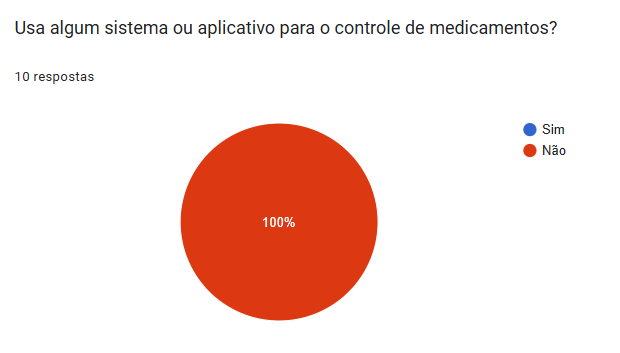
\includegraphics[width=0.75\linewidth]{Figuras/utiliza-app.png}
    \caption{Pergunta 6/10}
    \fonte{Autores.}
    \label{utiliza_app}
\end{figure}

\begin{figure}[!htbp]
    \centering
    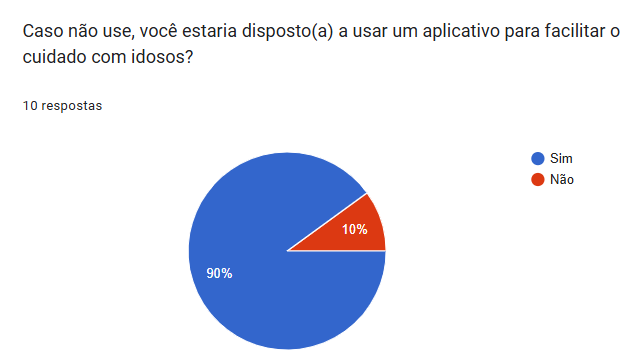
\includegraphics[width=0.75\linewidth]{Figuras/utilizaria-app.png}
    \caption{Pergunta 9/10}
    \fonte{Autores.}
    \label{utilizaria_app}
\end{figure}

\subsection{Ferramentas e Tecnologias}

Para a organização e acompanhamento do desenvolvimento, foi adotada uma abordagem baseada no framework Scrum, adaptada à realidade e às necessidades da equipe. O processo foi estruturado em sprints com duração de quatro semanas, com reuniões semanais para alinhamento das tarefas e revisão do progresso. As tarefas foram gerenciadas no Jira, permitindo o acompanhamento visual do fluxo de trabalho e facilitando a priorização das entregas. Essa adaptação do Scrum proporcionou maior autonomia à equipe, mantendo a organização e o foco nos objetivos do projeto.

Durante o desenvolvimento do \nomeprojeto, foram selecionadas tecnologias e ferramentas que garantem escalabilidade e facilidade de manutenção. No back-end, utilizou-se o MySQL como Sistema Gerenciador de Banco de Dados (SGBD) devido à sua confiabilidade, aliado ao framework Spring Boot em Java, que facilita a criação de APIs RESTful e a integração com outros serviços.

No front-end, optou-se pelo Angular 19, que permite o desenvolvimento de interfaces dinâmicas e reativas através de componentes. A biblioteca de componentes PrimeNG e a linguagem de design Material Design 3 foram incorporados para padronizar o design da aplicação. Para autenticação e autorização, foi utilizado o Auth0, que oferece uma solução segura e prática de Single Sign On (SSO).

Durante o desenvolvimento, o Visual Studio Code (VSCode) foi escolhido como editor de código por sua leveza, extensibilidade e integração com diversas ferramentas. O controle de versão foi realizado com o Git, utilizando o GitHub para hospedagem dos repositórios e o GitKraken para facilitar a gestão de branches e colaboração entre os membros da equipe.

A gestão de tarefas e acompanhamento do progresso do projeto foi feita com o Jira, permitindo organização eficiente das entregas e reuniões. Por fim, o Google Workspace foi utilizado para armazenamento e compartilhamento de documentos, além de servir como plataforma para aplicação dos formulários de pesquisa, através das aplicações Google Drive, Google Docs, Google Forms e Google Sheets.
	
\subsection{Processo de Desenvolvimento}

Em primeira instância, foi desenvolvido o back-end a partir da modelagem proposta, criando o banco de dados em SQL, e hospedando-o na Google Cloud Platform. O desenvolvimento do back-end e integração com banco de dados foi desenvolvida com Java e Spring Boot, e hospedada na plataforma Render.

Para o desenvolvimento do front-end, utilizou-se Angular 19 para a criação de páginas reativas, que mudam de estado. A biblioteca PrimeNG é usada para facilitar a criação de estilos dos elementos e simplificar a componentização e redução do código. Para a hospedagem, foi escolhida a plataforma Firebase.

Recursos externos foram utilizados para coleta de dados, a API "api-medicamentos-anvisa", hospedada publicamente oferece nomes e informações úteis de todos os medicamentos registrados no Brasil até 2020. Além dela, a API de busca do Google foi utilizada por meio da ferramenta "SerperDev", da qual oferece uma interface simples à pesquisa de locais e produtos farmacêuticos.

\subsection{Equipe}

O desenvolvimento do \nomeprojeto\ se deu pela estruturação do projeto em equipe, após isso houve a designação de responsabilidades para cada colaborador. Esta seção diz sobre a organização de forma ampla e a alocação de tarefas.

O \autoref{quadro_integrantes} discorre a respeito da distribuição de tarefas da equipe. Para cada segmento do projeto foram designados ao mínimo duas pessoas, a fim de obter uma visão mais ampla de desenvolvimento; com exceção da execução de testes, que por sua natureza exige menos atenção. 

\begin{quadro}
    \caption{\label{quadro_integrantes}Integrantes da equipe}
        \begin{tabular}{|c|c|c|c|c|c|c|}
        \hline
            Papéis         & Arthur                    & Fernando                  & Henriquy                  & Isabella                  & Lucas                     & Mateus                    \\ \hline
            Back-end       &                           &                           &                 &                           & \checkmark                & \checkmark                \\ \hline
            Front-end      & \checkmark                & \checkmark                &                           & \checkmark                &                           &                           \\ \hline
            Banco de Dados &                           &                           & \checkmark                &                           & \checkmark                &                           \\ \hline
	        Testes 	   &			       & 			   & \checkmark		       & 			   & 			       &			   \\ \hline
            Documentação   & \checkmark                & \checkmark                & \checkmark                & \checkmark                & \checkmark                & \checkmark                \\ \hline
            Design         &                           &                           & \checkmark                & \checkmark                &                           &                           \\ \hline
            Gestão         &                           &                           & \checkmark                &                           & \checkmark                &                           \\ \hline
        \end{tabular}
    \fonte{Autores.}
\end{quadro}

\section{Desenvolvimento}

Esta seção percorre todas as etapas do desenvolvimento do projeto, desde sua projeção de requisitos de funcionamento e regras de negócio, modelagem e prototipagem e testes.

\subsection{Requisitos}

Os requisitos do sistema, divididos em funcionais e não funcionais, detalham os recursos e as características planejadas para o projeto. A definição de cada requisito foi baseada na análise das pesquisas realizadas com o público-alvo e na avaliação da viabilidade de desenvolvimento.

\subsubsection{Requisitos Funcionais}

Requisitos funcionais são especificações que descrevem as funcionalidades e comportamentos que um sistema deve possuir para atender às necessidades dos usuários, definindo o que o sistema deve fazer e detalhando as interações entre o usuário e o software.

O requisito funcional RF04 (Notificações), criado para garantir que os usuários sejam alertados sobre eventos importantes, como horários de medicação ou consultas agendadas, o requisito funcional RF07 (Relatórios), criado para garantir que os usuários possam acompanhar a evolução clínica de pacientes por meio de relatórios detalhados e o requisito funcional RF10 (Log), incluído para registrar logs de acesso e operações críticas, como edições ou exclusões, são requisitos essenciais para garantir que o sistema atenda aos objetivos propostos e forneça valor ao público-alvo. 

Esses três itens surgiram a partir da síntese das pesquisas tanto com o público geral quanto com o público alvo da aplicação, identificando dores dos usuários e como o sistema pode ajudá-los a solucionar esses problemas. O \autoref{requisitos_f} mostra todos os requisitos funcionais criados para o \nomeprojeto.

\subsubsection{Requisitos Não-Funcionais}

Requisitos não-funcionais são especificações que descrevem as características e restrições de qualidade que o sistema deve atender para garantir sua eficiência, segurança e usabilidade. Esses requisitos não estão diretamente relacionados às funcionalidades do sistema, mas são essenciais para que ele opere de forma confiável e atenda às expectativas dos usuários.

O requisito não-funcional RNF01 (Segurança), criado para assegurar a criptografia de dados sensíveis, como senhas e informações médicas, é essencial para proteger a privacidade dos usuários e garantir conformidade com regulamentações como a LGPD. O requisito RNF06 (Desempenho), que define que o sistema deve responder às requisições em até, no máximo, 1,5 segundos, foi incluído para garantir uma experiência fluida e eficiente, especialmente em operações críticas. Já o requisito RNF10 (Disponibilidade), que exige que o sistema permaneça disponível pelo menos 99,5\% do tempo durante o horário de operação, é fundamental para assegurar que os usuários possam acessar o sistema sempre que necessário, minimizando interrupções.

Esses três requisitos foram definidos com base nas melhores práticas de desenvolvimento de software, como padrões para APIs RESTful, e nas necessidades identificadas durante a análise do público-alvo junto a reflexão sobre os requisitos funcionais. O \autoref{requisitos_nf} apresenta todos os requisitos não-funcionais criados para o sistema.

\subsection{Regras de Negócio}

Regras de negócio são diretrizes que definem como o sistema deve operar em situações específicas, garantindo que os processos sigam padrões estabelecidos. Elas são fundamentais para assegurar que o sistema funcione de maneira consistente e em conformidade com as regulamentações aplicáveis.

A regra de negócio RN02 (Segurança), que determina o arquivamento de registros excluídos por 15 dias antes da remoção definitiva, foi incluída para atender às exigências da LGPD, inclusive para permitir que os usuários tenham tempo para reverter os pedidos de exclusão ou recuperar alguma informação. A regra RN04 (Tratamentos), que exige que a conclusão ou o cancelamento de tratamentos seja realizado apenas por cuidadores autorizados e registrado em log, foi definida para garantir rastreabilidade e controle sobre ações sensíveis no sistema. Já a regra RN07 (Segurança) foi adicionada para garantir que todas informações pertencentes a um usuário devem ser armazenadas de forma segura e criptografada, a fim de respeitar normas de segurança.

Essas regras foram elaboradas com base nas necessidades do público alvo e nas regulamentações aplicáveis, como a LGPD, para garantir que o sistema seja seguro e confiável. O \autoref{regras_negocio} apresenta todas as regras de negócio definidas para a aplicação.

\subsection{Modelagem}

A modelagem do sistema é uma etapa fundamental que visa traduzir os requisitos e regras de negócio em uma representação estruturada do software. Este processo envolve os casos de uso, a definição da arquitetura, e a estrutura de dados da aplicação. Para o \nomeprojeto, a modelagem foi detalhada por meio de diagramas s de uso, que descrevem as interações entre os usuários e o sistema, o diagrama de arquitetura de sistema, que descreve como o sistema está estuturado tecnicamente e pelo modelo de entidade e relacionamento, que detalha a estrutura do banco de dados.

\subsubsection{Casos de Uso}

Como apresentado na \autoref{casos_de_uso}, os casos de uso representam as principais interações entre os usuários e o sistema, descrevendo como as funcionalidades foram projetadas para atender às necessidades identificadas durante a análise de requisitos. Eles são fundamentais para garantir que o sistema seja desenvolvido de forma alinhada às expectativas do público-alvo e às regras de negócio definidas.

\begin{figure}[!htbp]
    \centering
    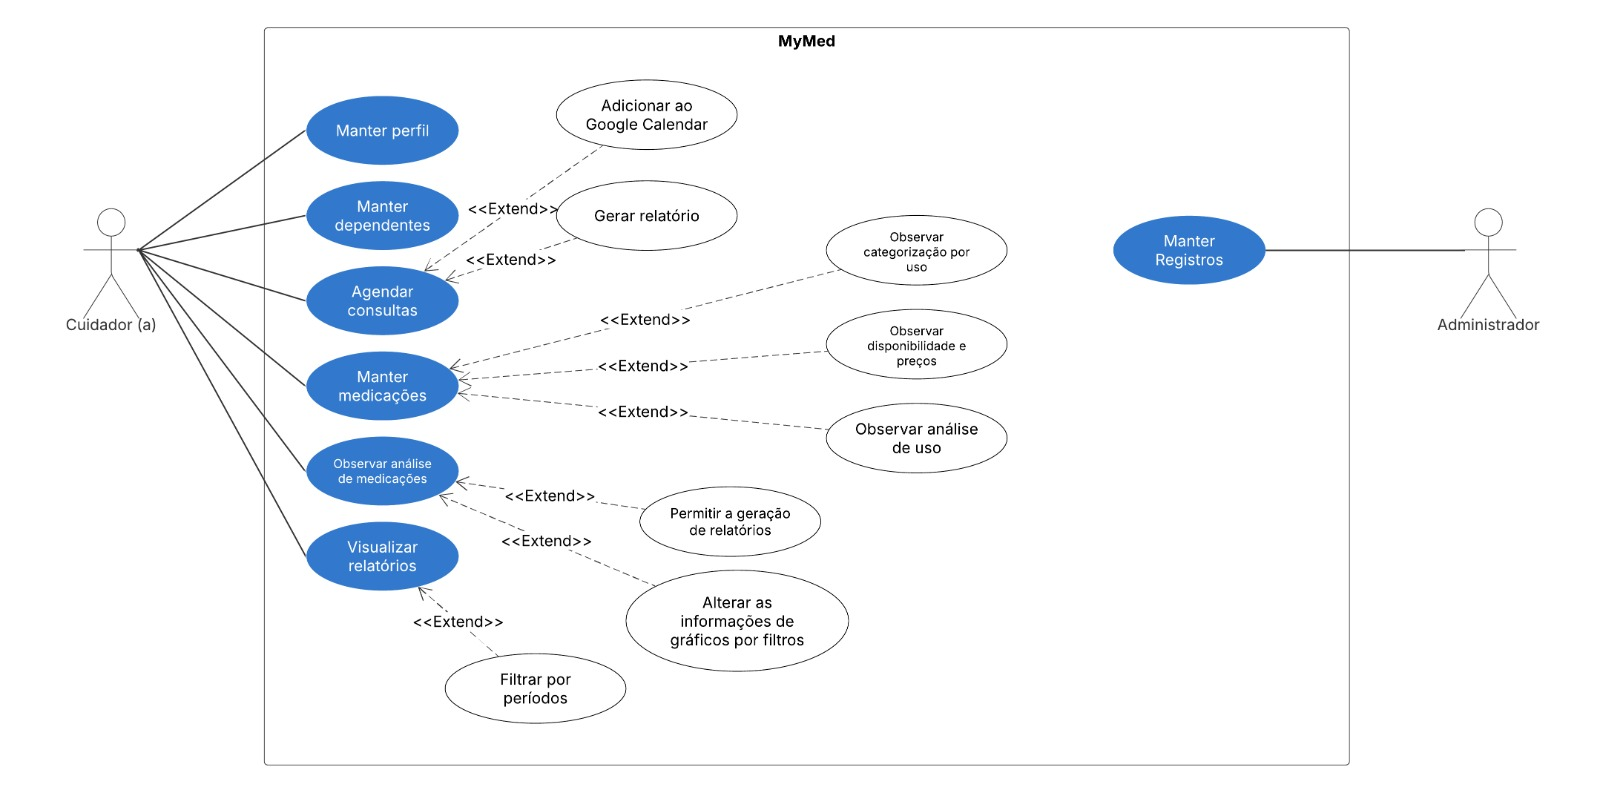
\includegraphics[width=1.0\linewidth]{Figuras/diagrama-casos-uso.jpg}
    \caption{Diagrama de Casos de Uso}
    \fonte{Autores.}
    \label{casos_de_uso}
\end{figure}


No \nomeprojeto, os casos de uso foram elaborados para cobrir as principais operações realizadas pelos cuidadores e administradores. Entre os casos de uso mais relevantes, destacam-se o caso de uso "Manter Dependentes" permite que o cuidador adicione, visualize, edite e exclua informações dos pacientes, garantindo que os dados estejam sempre atualizados. Já o caso de uso "Agendar Consulta" possibilita que o cuidador registre compromissos médicos em uma agenda para os pacientes, com integração opcional ao calendário do dispositivo. Além disso, o caso de uso "Gerenciar Medicações" permite o acompanhamento do estoque de medicamentos e o registro de consumo, emitindo alertas em caso de baixa disponibilidade.

O \autoref{dicionario_casos_uso} apresenta o \textit{Dicionário de Casos de Uso}, apresentando cada cenário com detalhes e informações sobre os atores envolvidos, pré-condições, fluxos principais e pós-condições.


\newpage

\subsubsection{Modelo Entidade Relacionamento}

O MER do MyMed foi projetado para representar as principais entidades do sistema, como Usuário, Dependente, Consulta, Tratamento e Medicação, além de suas relações. Ele garante que as informações sejam armazenadas de forma consistente e que as interações entre as entidades sejam bem definidas. A \autoref{model_entidade_relacionamento} apresenta o diagrama completo, detalhando as entidades e seus relacionamentos.

\begin{figure}[!htbp]
    \centering
    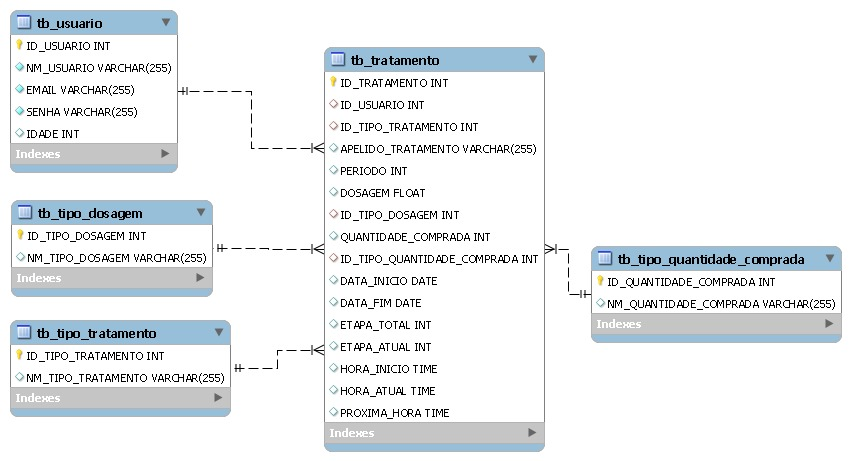
\includegraphics[width=1.0\linewidth]{Figuras/bancoDados.jpg}
    \caption{Imagem do Modelo Entidade Relacionamento}
    \fonte{Autores.}
    \label{model_entidade_relacionamento}
\end{figure}

Por exemplo, a entidade Usuário está relacionada à entidade Dependente, permitindo que cuidadores gerenciem os dados de seus dependentes. A entidade Consulta está associada tanto ao Usuário quanto ao Dependente, possibilitando o registro de compromissos médicos para ambos. Já a entidade Tratamento está vinculada a Medicação, permitindo o acompanhamento detalhado de medicamentos prescritos e consumidos.

O MER reflete a necessidade de um sistema robusto e escalável, garantindo que os dados sejam organizados de forma eficiente e que as operações, como consultas e atualizações, sejam realizadas de maneira confiável. Ele também assegura a integridade referencial, evitando inconsistências nos dados e permitindo que o sistema atenda aos requisitos funcionais e não funcionais definidos. 

\newpage

\subsection{Arquitetura de Software}

Esta subseção apresenta a arquitetura geral do sistema, suas tecnologias, infraestrutura de hospedagem e os fluxos de interação entre os contêineres. O modelo utilizado é baseado no \textit{Diagrama de Contêineres do C4 Model}.

\subsubsection{Visão Geral}

A arquitetura do sistema é composta por quatro contêineres principais, cada um com responsabilidades específicas e hospedado em diferentes plataformas de nuvem. Essa estrutura foi definida visando escalabilidade, isolamento de responsabilidades e maior confiabilidade.

A comunicação entre esses contêineres ocorre predominantemente por meio de requisições HTTP.

\begin{figure}[h!]
    \centering
    \caption{Diagramas da Arquitetura de Software}
    \begin{subfigure}[b]{0.45\textwidth}
        \centering
        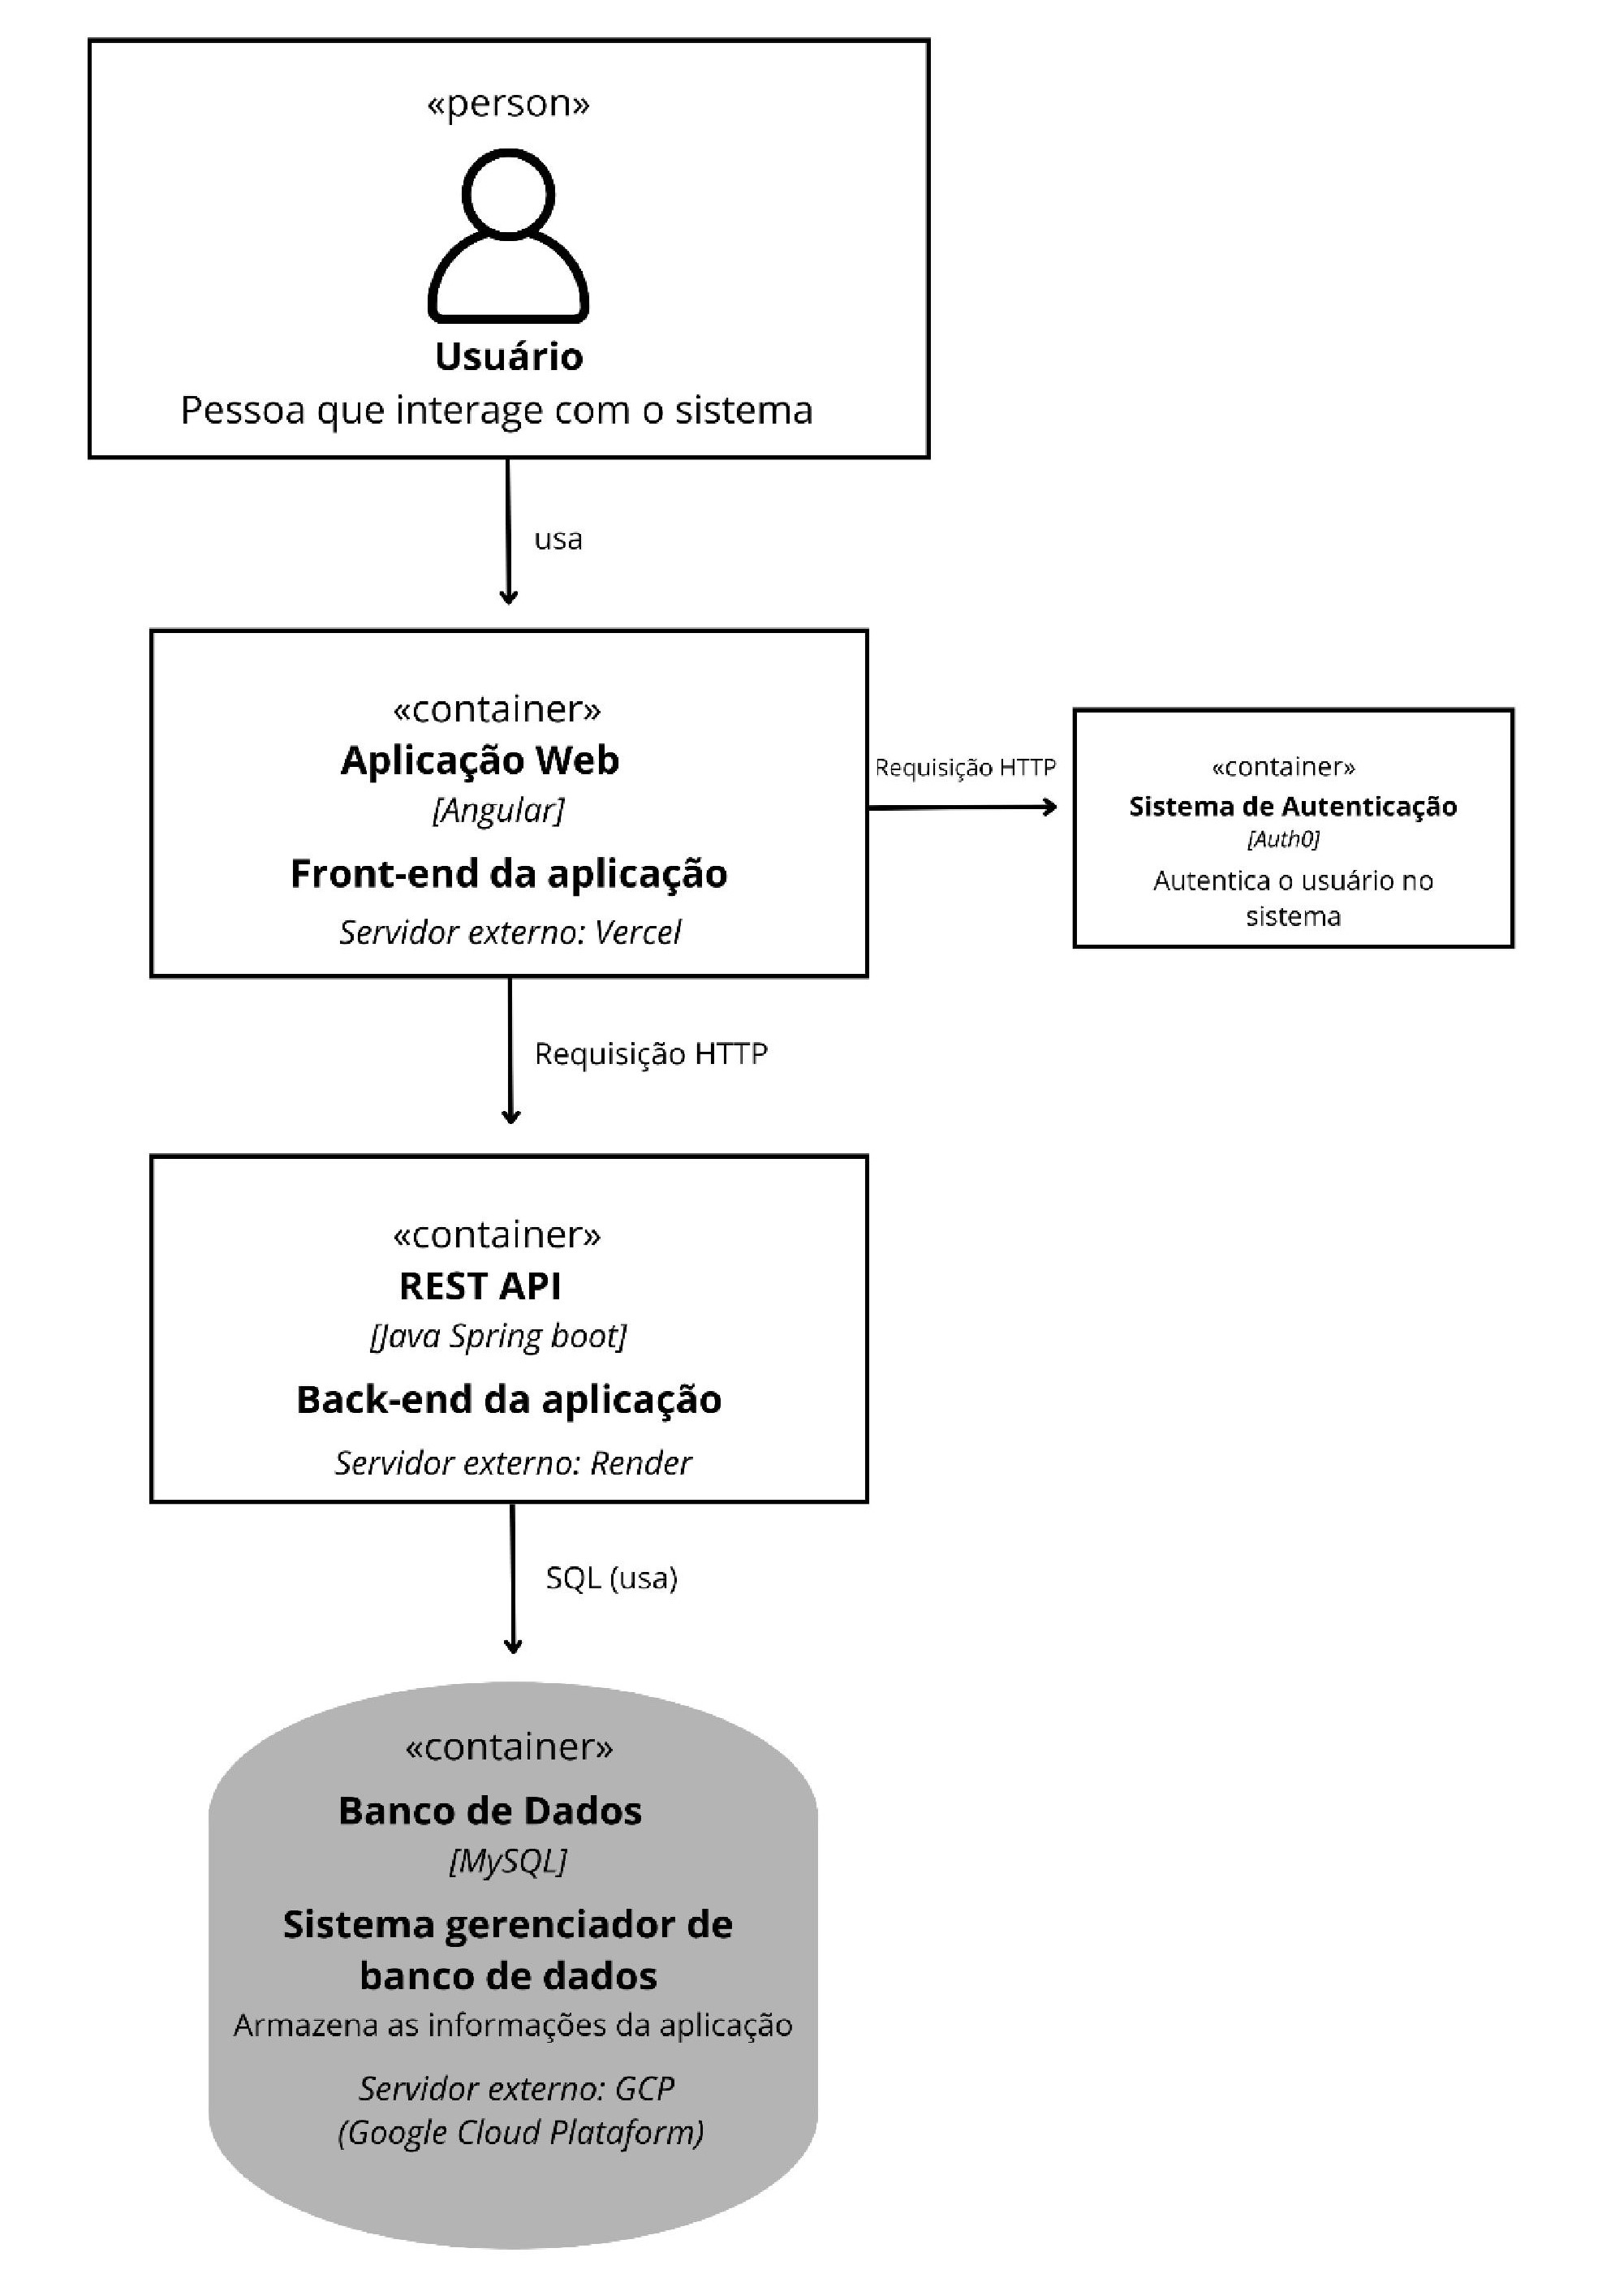
\includegraphics[width=\textwidth]{Figuras/diagrama_conteineres.jpg}
        \caption{Diagrama de Contêineres}
        \label{fig:diagrama-conteineres}
    \end{subfigure}
    \hfill
    \begin{subfigure}[b]{0.45\textwidth}
        \centering
        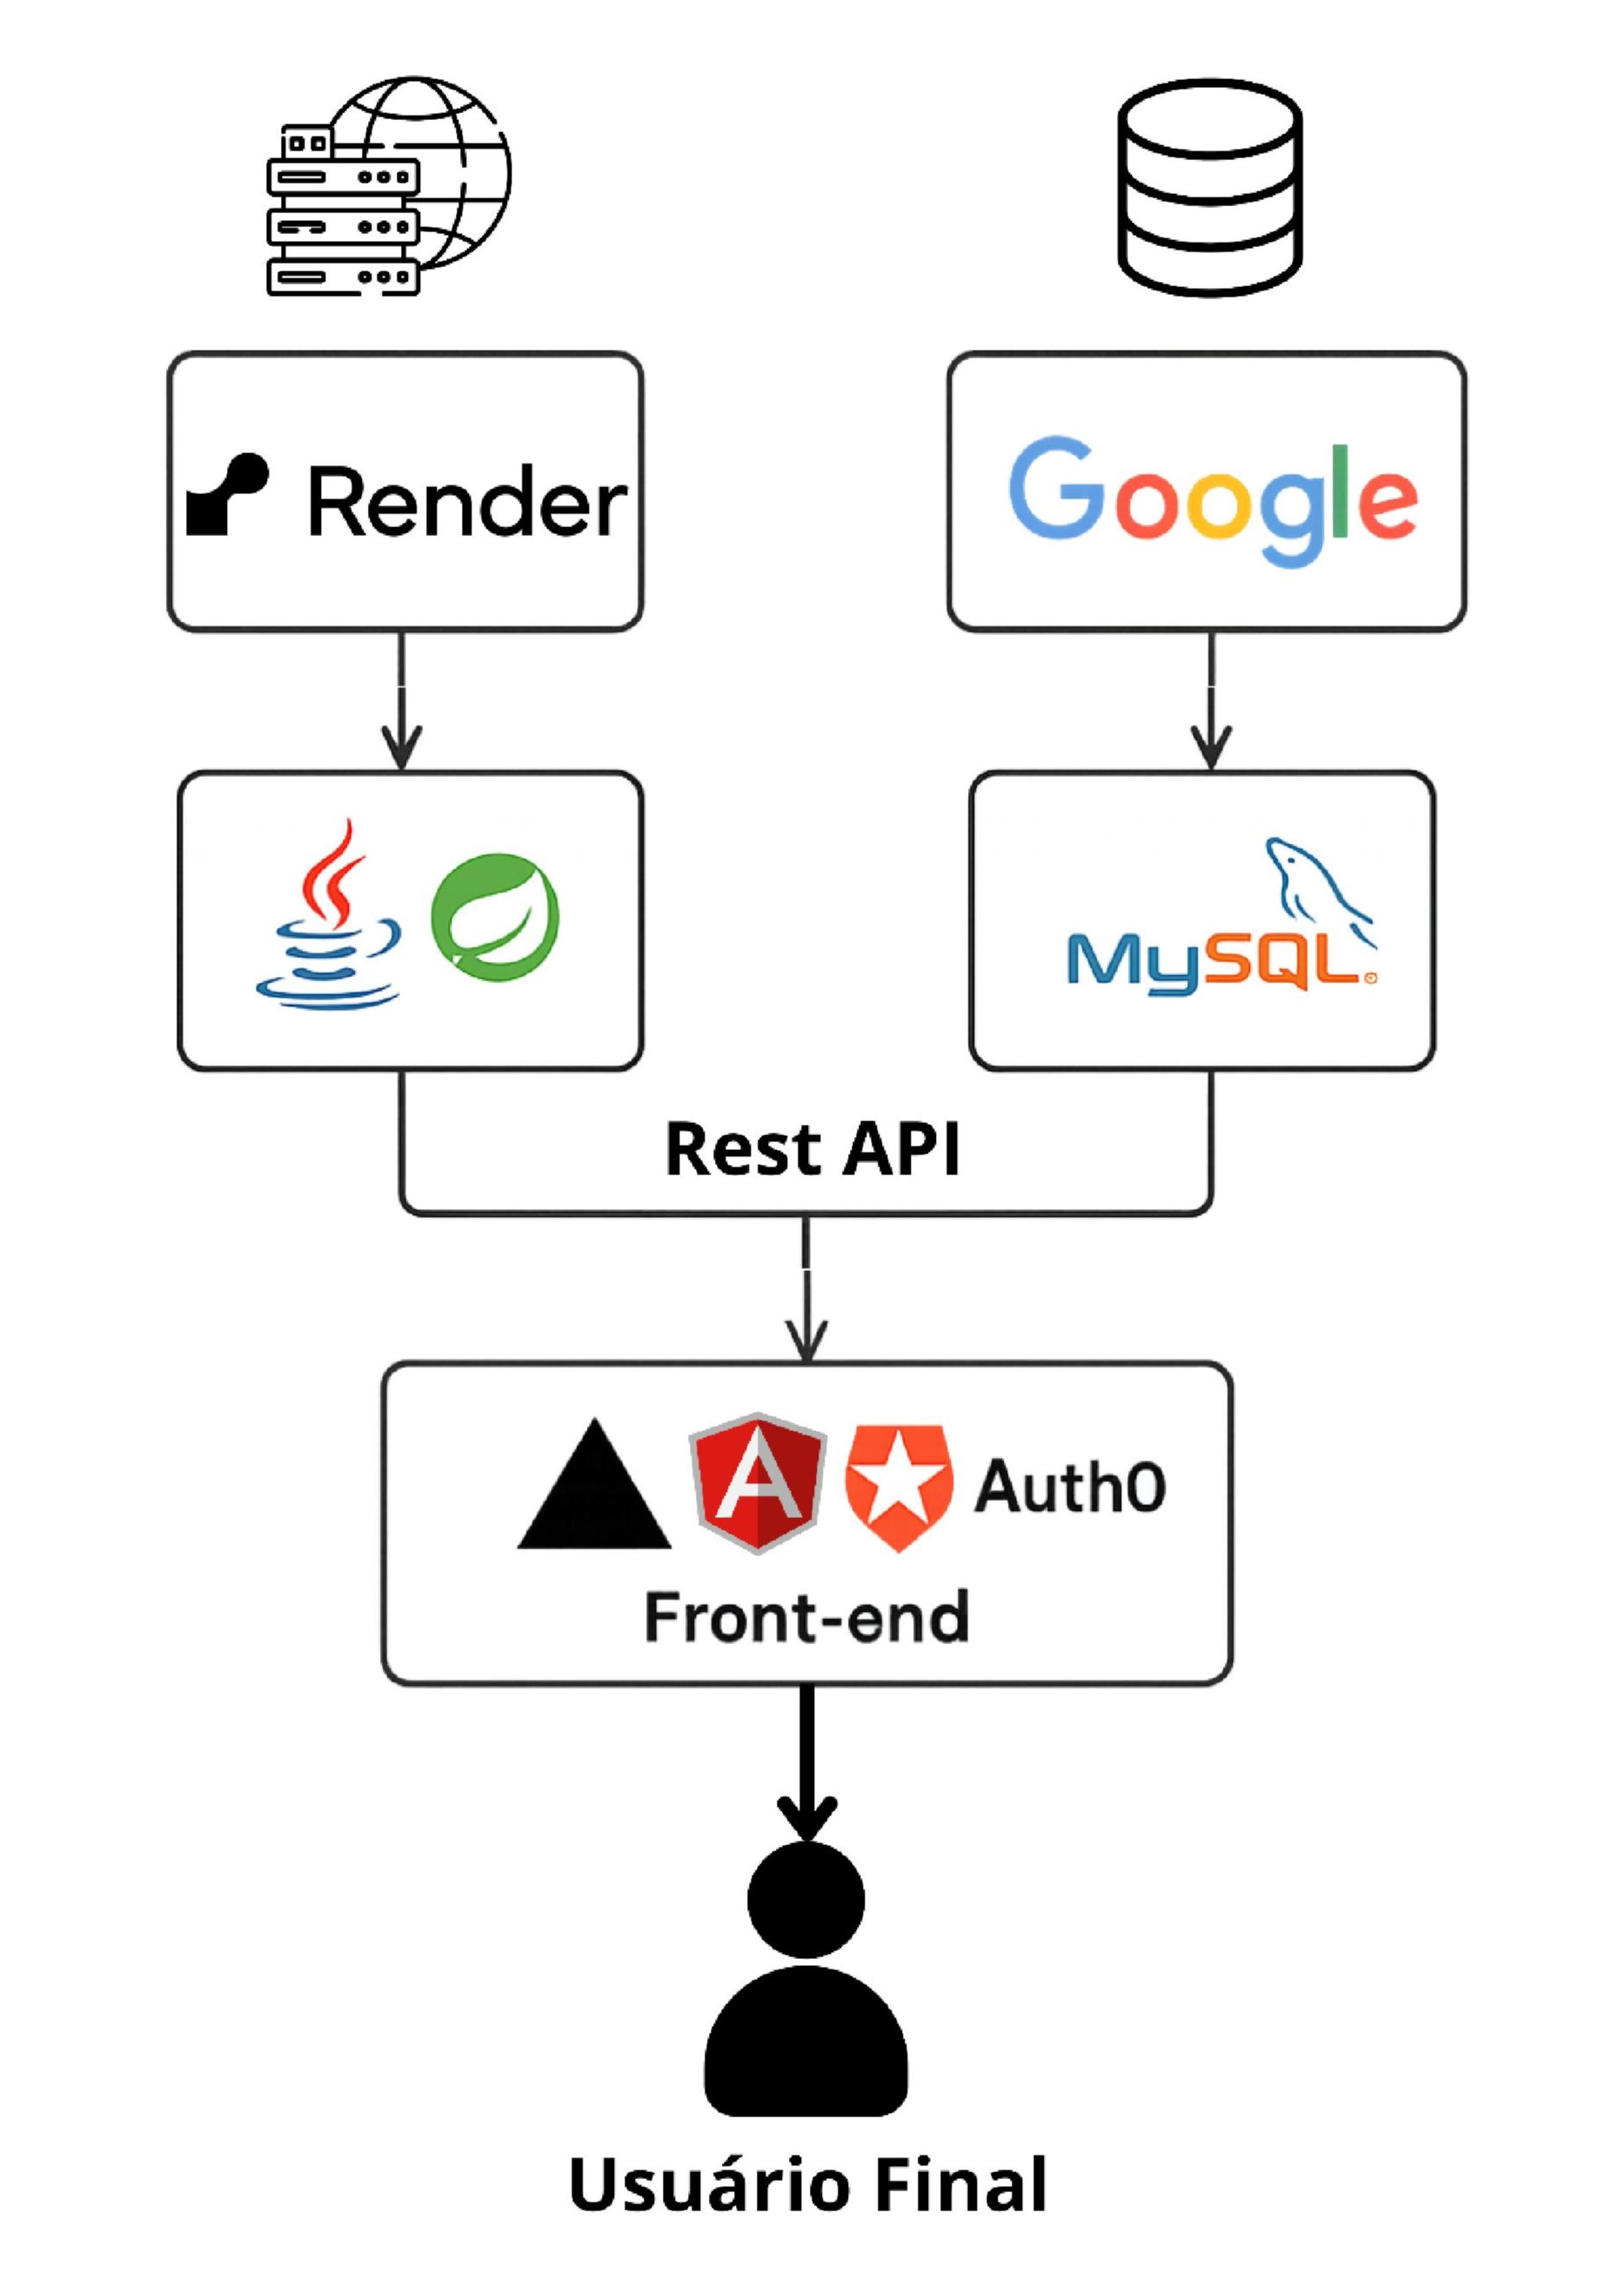
\includegraphics[width=\textwidth]{Figuras/fluxo_comunicacao.jpg}
        \caption{Fluxo de Comunicação}
        \label{fig:fluxo-comunicacao}
    \end{subfigure}
    \label{fig:arquitetura-software}
    \fonte{Autores.}
\end{figure}

\subsubsection{Detalhamento dos Contêineres}

\textbf{Usuário}\\
\textit{Tipo:} Pessoa.\\
\textit{Descrição:} Representa o usuário final que interage com o sistema por meio da aplicação web.

\textbf{Aplicação Web (Front-end)}\\
\textit{Tipo:} Contêiner.\\
\textit{Tecnologia:} Angular.\\
\textit{Descrição:} Interface responsável por apresentar informações e funcionalidades ao usuário de forma acessível.\\
\textit{Infraestrutura:} Hospedada na plataforma Vercel.\\
\textit{Interação:} Comunicação via HTTP com a REST API e o sistema de autenticação.

\textbf{REST API (Back-end)}\\
\textit{Tipo:} Contêiner.\\
\textit{Tecnologia:} Java Spring Boot.\\
\textit{Descrição:} Responsável por processar as regras de negócio da aplicação e interagir com o banco de dados.\\
\textit{Infraestrutura:} Hospedada na plataforma Render.\\
\textit{Interação:} Recebe requisições HTTP da aplicação web e acessa o banco de dados via SQL.

\textbf{Banco de Dados}\\
\textit{Tipo:} Contêiner.\\
\textit{Tecnologia:} MySQL.\\
\textit{Descrição:} Responsável pelo armazenamento persistente das informações da aplicação.\\
\textit{Infraestrutura:} Hospedado na Google Cloud Platform (GCP).\\
\textit{Interação:} Acesso exclusivo pela REST API.

\textbf{Sistema de Autenticação}\\
\textit{Tipo:} Contêiner.\\
\textit{Tecnologia:} Auth0.\\
\textit{Descrição:} Serviço responsável por autenticar os usuários e controlar o acesso ao sistema.\\
\textit{Infraestrutura:} Serviço externo SaaS.\\
\textit{Interação:} Comunicação via HTTP com a aplicação web.

\subsubsection{Fluxo de Operação}

\begin{enumerate}
    \item O usuário acessa a aplicação web hospedada na Vercel.
    \item A aplicação web realiza requisições HTTP ao sistema de autenticação (Auth0) para autenticar o usuário.
    \item Após a autenticação, a aplicação envia requisições HTTP para a REST API hospedada na Render, solicitando operações de negócio.
    \item A REST API processa as solicitações e interage com o banco de dados MySQL hospedado na GCP via SQL.
    \item As respostas do banco de dados são processadas pela REST API e devolvidas à aplicação web, que as apresenta ao usuário final.
\end{enumerate}

\subsection{Prototipagem}

A prototipagem do sistema se deu pela criação inicial do conceito do sistema e fluxos de dados, depois foi feito o design das telas de usuário na plataforma \textit{Figma}. Em anexo, há as telas feitas na plataforma, o \autoref{prototipagem} traz as telas do sistema, que são compostas pelas seguintes seções:

\begin{enumerate}
    \item \textbf{Tela inicial:} o usuário pode visualizar as informações gerais do sistema, como o estoque de medicamentos e os níveis de glicemia e pressão arterial;
    \item \textbf{Calendário:} o usuário pode visualizar as consultas agendadas e os medicamentos que devem ser consumidos naquele dia;
    \item \textbf{Gráfico:} o usuário pode visualizar os gráficos de níveis de glicemia e pressão arterial;
    \item \textbf{Consulta:} o usuário pode visualizar as consultas agendadas, além de poder criar novas consultas e editar as já existentes;
    \item \textbf{Perfil:} o usuário pode visualizar e editar seu perfil, além de poder adicionar dependentes e editar os já existentes;
\end{enumerate}

\subsection{Plano de Testes}

O plano de testes visa verificar todas as funcionalidades e validar seu uso na aplicação. O \autoref{quadro_testes} retrata todos os testes que devem ser implementados nos diversos segmentos do sitema, como a verificação da conexão com o banco de dados, validação de informações de usuário e exibição correta de consultas conforme a data do dispositivo.

\begin{quadro}
  \caption{\label{quadro_testes}Plano de Testes do Sistema \nomeprojeto}
    \begin{tabular}{|p{4cm}|p{5cm}|p{5cm}|}
      \hline
      \textbf{Objeto de Teste} & \textbf{Resultado Esperado} & \textbf{Possíveis Divergências} \\
      \hline
      Enviar usuário ao banco & Criação de usuário no banco de dados & A conexão com o banco de dados pode falhar \\
      \hline
      Enviar dependente ao banco & Criação de dependente no banco de dados & A conexão com o banco de dados pode falhar \\
      \hline
      Enviar consulta ao banco & Criação de consulta no banco de dados & A conexão com o banco de dados pode falhar \\
      \hline
    \end{tabular}
  \fonte{Autores.}
\end{quadro}

\subsection{Criptografia}

Para garantir a segurança na comunicação entre os usuários e a aplicação, foi configurado o protocolo HTTPS com suporte a TLS, utilizando certificados digitais válidos e atualizados. A certificação foi realizada através da integração com o serviço Let's Encrypt através do Render para o back-end e Gerenciado pelo Google para o front-end através do Firebase Hosting, assegurando criptografia ponta a ponta durante as transações de dados. A configuração foi validada na ferramenta SSL Labs, onde o ambiente obteve a nota máxima A+.

\begin{figure}[h!]
    \caption{Resultados dos testes de criptografia.}
    \centering
    \begin{subfigure}[b]{0.45\textwidth}
        \centering
        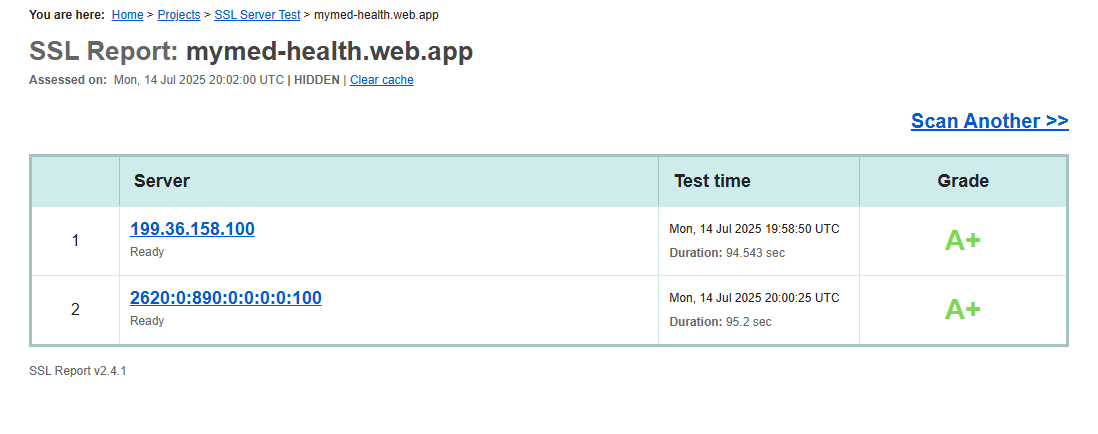
\includegraphics[width=\textwidth]{Figuras/certificacao_front.png}
        \caption{Resultado dos testes do front-end}
    \end{subfigure}
    \hfill
    \begin{subfigure}[b]{0.45\textwidth}
        \centering
        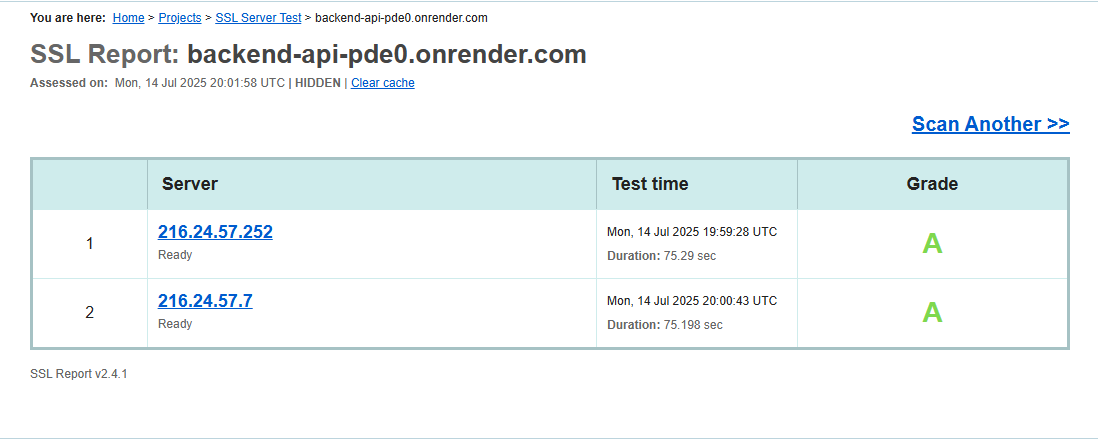
\includegraphics[width=\textwidth]{Figuras/certificacao_back.png}
        \caption{Resultado dos testes do back-end}
    \end{subfigure}
    \label{fig:testes-criptografia}
     \fonte{Autores.}
\end{figure}

\section{MVP}

O termo MVP foi popularizado por  \citeonline{ries2011lean}, onde ele descreve o conceito como segue:

"O MVP é o menor conjunto de recursos que permite que o empreendedor comece o processo de aprendizado com o mínimo de esforço e o máximo de aprendizado validado sobre os clientes."

Outro autor importante na área, \citeonline{blank2013startup}, define o MVP como:

"Uma ferramenta para testar hipóteses de negócios e iniciar o aprendizado, coletando o máximo de informações validadas sobre os clientes com o menor esforço possível."


% ---
% Finaliza a parte no bookmark do PDF, para que se inicie o bookmark na raiz
% ---
\bookmarksetup{startatroot}% 
% ---

% ---
% Conclusão
% ---
\section{Considerações finais}

De acordo com \citeonline{severino2016metodologia}, na seção de considerações finais o autor tem a oportunidade de fazer uma síntese dos principais pontos abordados e apresentar suas considerações finais sobre o assunto. Embora não haja uma estrutura fixa, existem algumas diretrizes comuns para escrever essa seção.

A seguir, algumas orientações gerais, para complementar a explicação:

1. Recapitule os principais pontos: Na seção de considerações finais, você pode revisitar os principais pontos discutidos ao longo do trabalho e resumir os resultados obtidos. É uma oportunidade para destacar a relevância do estudo e como ele contribui para o conhecimento existente.

2. Discuta as implicações dos resultados: Nessa seção, você pode discutir as implicações práticas e teóricas dos resultados do seu trabalho. 

3. Faça uma reflexão crítica: Use a seção de considerações finais para fazer uma reflexão crítica sobre as limitações do estudo e possíveis viéses. Discuta as dificuldades encontradas, bem como eventuais lacunas de conhecimento que podem ser exploradas por estudos futuros.

4. Encerre de forma concisa e impactante: Finalize a seção de considerações finais com uma frase ou parágrafo que resuma as principais conclusões e destaque a importância do estudo. É uma oportunidade para deixar uma impressão duradoura nos leitores.

% ----------------------------------------------------------
% ELEMENTOS PÓS-TEXTUAIS
% ----------------------------------------------------------
\postextual

% ----------------------------------------------------------
% Referências bibliográficas
% ----------------------------------------------------------

% ----------------------------------------------------------
% Glossário
% ----------------------------------------------------------
%
% Há diversas soluções prontas para glossário em LaTeX. 
% Consulte o manual do abnTeX2 para obter sugestões.
%
% \glossary
% ----------------------------------------------------------
% Apêndices
% ----------------------------------------------------------

\bibliography{referencias}
% ---
% Inicia os apêndices
% ---
\newpage
\begin{apendicesenv}

% % % % ----------------------------------------------------------
\chapter{Pesquisas\label{pesquisas}}

As pesquisas foram conduzidas para entender melhor as necessidades e desafios enfrentados pelos usuários e cuidadores de idosos. A seguir, apresentamos as perguntas formuladas para cada grupo respectivo. Os formulários foram aplicados por meio don Google Forms, garantindo a coleta de dados de forma organizada e acessível.

\section{Pesquisa com o Público Geral}
\begin{enumerate}
    \item Se não se importar, poderia informar o seu nome? (a resposta não é obrigatória)
    \item Você já utilizou alguma aplicação ou sistema de auxílio no gerenciamento de medicamentos/consultas? (Sim ou Não)
    \item Se sim, se importa de compartilhar sua experiência? Como é o aplicativo? (Resposta livre)
    \item Você possui alguma dificuldade ao lidar com tratamentos com remédios? (Lembrar os horários, Dosagens, Reposição dos remédios, Nenhuma)
    \item Você possui alguma dificuldade ao lidar com vacinas? (Lembrar as datas, Disponibilidade, Nenhuma)
    \item Você possui alguma dificuldade ao lidar com consultas? (Lembrar a data e/ou horário de agendamento, Organização, Nenhuma)
    \item No momento atual, o que você considera sua maior dificuldade ao gerenciar seus tratamentos e/ou compromissos médicos? (Resposta livre)
    \item Já utilizou algum serviço de Teleconsulta? (Sim ou Não)
    \item Se sim, se importa de compartilhar sua experiência? Foi positiva ou negativa? (Resposta livre)
    \item Já utilizou algum serviço de Tele-educação voltado à área da saúde? (Sim ou Não)
    \item Se sim, se importa de compartilhar sua experiência? Foi positiva ou negativa? (Resposta livre)
    \item Consegue dizer um processo, que se fosse automático, auxiliaria você no gerenciamento de seus compromissos médicos nos dias atuais? Se sim qual? (Resposta livre)
\end{enumerate}

\section{Pesquisa com Cuidadores de Idosos}
\begin{enumerate}
    \item Qual sua função atual? (Cuidador(a), Coordenador(a), Enfermeiro(a), Outros)
    \item Você trabalha em: (Asilo, Casa de repouso, Domicílio particular, Outros)
    \item Quantos idosos você(s) cuida(m) atualmente? (1-5, 5-20, 20-50, 50+)
    \item Quais atividades fazem parte da sua rotina com os idosos? [Marque todas que se aplicam] (Administração de medicamentos, Monitoramento de sinais vitais, Acompanhamento em consulta, Outros)
    \item Como você organiza os horários e dosagens dos medicamentos dos idosos? (Resposta livre)
    \item Usa algum sistema ou aplicativo para o controle de medicamentos? (Sim ou Não)
    \item Se sim, qual? (Resposta livre)
    \item Como você registra a rotina e as informações de saúde dos idosos? [Marque todas que se aplicam] (Aplicativos ou softwares, Papel, Planilhas (Excel, Google Sheets), Não Registro)
    \item Caso não use, você estaria disposto(a) a usar um aplicativo para facilitar o cuidado com idosos? (Sim ou Não)
    \item O que esse app deveria ter para ser útil no seu dia a dia? (Resposta livre)
\end{enumerate}


\newpage

\chapter{Requisitos Funcionais\label{requisitos_f}}

Os requisitos funcionais são essenciais para definir as funcionalidades que o sistema deve oferecer, garantindo que atenda às necessidades dos usuários e aos objetivos do negócio. A seguir, apresentamos uma tabela com os principais requisitos funcionais definidos para o sistema de gestão de dependentes.

\begin{longtblr}[
  label = requisitos_f,
  entry = none,
  caption = {Requisitos Funcionais},
  note = {Fonte: Autores.},
]{
  vline{1-4} = {-}{},
  hline{-} = {1-3}{},
}
Código & Categoria    & Descrição                                                                                       &  \\
RF01   & Cadastro     & {Cadastrar paciente: dados pessoais \\(nome, CPF, data de nascimento, endereço, contato, etc.)} &  \\
RF02   & Paciente     & {Visualizar perfil do paciente: \\histórico de atendimentos e tratamentos}                      &  \\
RF03   & Paciente     & Editar e atualizar dados do paciente                                                            &  \\
RF04   & Cadastro     & {Excluir cadastro de paciente: \\mas mantendo o histórico arquivado}                            &  \\
RF05   & Consulta     & {Agendar nova consulta: \\paciente, profissional, data, hora e local}                           &  \\
RF06   & Consulta     & {Listar consultas agendadas:\\~com filtros por data, profissional ou paciente}                  &  \\
RF07   & Consulta     & {Editar ou cancelar consulta: \\antes da data marcada}                                          &  \\
RF08   & Atendimento  & {Registrar atendimento: \\diagnóstico, conduta, recomendações, etc}                             &  \\
RF09   & Notificação  & {Emitir alertas ou notificações:\\~consultas futuras}                                           &  \\
RF10   & Tratamento   & {Criar plano de tratamento: \\associado a um paciente e diagnóstico}                            &  \\
RF11   & Tratamento   & {Listar tratamentos em andamento,\\concluídos ou cancelados (tipo kanban)}                      &  \\
RF12   & Tratamento   & {Registrar evolução do tratamento: \\observações por etapa ou sessão}                           &  \\
RF13   & Tratamento   & {Anexar prescrições médicas: \\laudos, imagens ou documentos ao tratamento}                     &  \\
RF14   & Relatório    & {Gerar relatórios de acompanhamento:\\paciente, profissional ou período}                        &  \\
RF15   & Histórico    & {Visualizar histórico de consultas: \\evolução clínica}                                         &  \\
RF16   & Exportação   & {Exportar dados: \\PDF, Excel ou outro formato}                                                 &  \\
RF17   & Autenticação & {Autenticar usuários: \\login e senha}                                                          &  \\
RF18   & Permissão    & {Gerenciar permissões: \\admin, profissional de saúde, recepcionista, etc}                      &  \\
RF19   & Log          & {Registrar logs de acesso:\\operações críticas (como edições e exclusões)}                      &  \\
RF20   & Pesquisa     & {Pesquisar pacientes, consultas e tratamentos:\\múltiplos critérios}                            &  \\
RF21   & Filtro       & Aplicar filtros e ordenações nas pesquisas                                                      &  
\end{longtblr}
\fonte{Autores.}

\newpage

\chapter{Requisitos Não Funcionais\label{requisitos_nf}}

Os requisitos não funcionais são igualmente importantes, pois definem as qualidades e restrições que o sistema deve atender, como segurança, desempenho e usabilidade. A seguir, apresentamos uma tabela com os principais requisitos não funcionais definidos para o sistema de gestão de dependentes.

\begin{quadro}
\caption{Requisitos Não-Funcionais do MyMed}
\begin{tabularx}{\textwidth}{|l|l|X|}
\hline
\textbf{Código} & \textbf{Categoria} & \textbf{Descrição} \\ \hline
RNF01 & Segurança & O sistema deve assegurar a criptografia de dados sensíveis, como senhas e informações médicas. \\ \hline
RNF02 & Acesso & O sistema deve implementar controle de acesso baseado em perfis de usuário, como administradores ou cuidadores. \\ \hline
RNF03 & Sessão & O sistema deve realizar a validação de sessão com expiração automática após período de inatividade. \\ \hline
RNF04 & Armazenamento & O sistema deve armazenar os dados de forma segura, em conformidade com a Lei Geral de Proteção de Dados (LGPD). \\ \hline
RNF05 & Backup & O sistema deve executar backups regulares e automáticos para possibilitar a recuperação de dados em caso de falha. \\ \hline
RNF06 & Desempenho & O sistema deve responder às requisições em até, no máximo 1,5 segundos durante as operações. \\ \hline
RNF07 & Interface & O sistema deve realizar paginação e carregamento sob demanda (lazy loading) em listas extensas, como consultas e pacientes. \\ \hline
RNF08 & Interface & O sistema deve possuir uma interface intuitiva e acessível para usuários sem conhecimento técnico. \\ \hline
RNF09 & Compatibilidade & O sistema deve ser compatível com dispositivos móveis, mantendo todas as funcionalidades acessíveis. \\ \hline
RNF10 & Disponibilidade & O sistema deve permanecer disponível pelo menos 99,5\% do tempo durante o horário de operação. \\ \hline
\end{tabularx}
\fonte{Autores.}
\end{quadro}

\newpage

\chapter{Regras de Negócio\label{regras_negocio}}

As regras de negócio são fundamentais para garantir o correto funcionamento do sistema, assegurando que as operações atendam aos requisitos legais e funcionais. A seguir, apresentamos uma tabela com as principais regras de negócio definidas para o sistema de gestão de dependentes.

\begin{longtblr}[
  label = regras_negocio,
  entry = none,
  caption = {Regras de Negócio},
  note = {Fonte: Autores.},
]{
  vline{1-4} = {-}{},
  hline{-} = {1-3}{},
}
Código & Categoria                      & Descrição                                                                                                                               &  \\
RN01   & Cadastro                       & {Apenas usuários com permissão de cuidador ou \\administrador podem cadastrar dependentes.}                                             &  \\
RN02   & Cadastro                       & {Cada dependente deve ter um \\CPF único e válido no sistema.}                                                                          &  \\
RN03   & Cadastro                       & {O sistema deve impedir o cadastro de dependentes \\com dados incompletos obrigatórios \\(ex: nome, CPF, data de nascimento, contato).} &  \\
RN04   & Cadastro                       & {A exclusão de um dependente não deve arquivar \\todo o histórico, porém não há \\remoção definitiva do banco de dados.}                &  \\
RN05   & Cadastro                       & {A edição de dados sensíveis (como CPF) \\deve ser registrada em log de auditoria.}                                                     &  \\
RN06   & Consultas                      & {Consultas só podem ser agendadas \\para dependentes cadastrados no sistema.}                                                           &  \\
RN07   & Consultas                      & {O sistema deve impedir agendamento\\de duas consultas no mesmo \\horário para o mesmo dependente.}                                     &  \\
RN08   & Consultas                      & {Consultas só podem ser editadas ou \\canceladas antes da data e hora marcadas.}                                                        &  \\
RN09   & Logs                           & {A edição ou exclusão de uma consulta\\criada deve ser registrada em log}                                                               &  \\
RN10   & Tratamentos                    & {Cada tratamento deve estar vinculado a um \\dependente específico e seu diagnóstico.}                                                  &  \\
RN11   & Tratamentos                    & {A evolução de um tratamento deve ser registrada \\com data, cuidador responsável e observações.}                                       &  \\
RN12   & Tratamentos                    & {Prescrições médicas devem ser anexadas com\\extensão válida (PDF, JPG, PNG, etc) \\e tamanho máximo pré-definido.}                     &  \\
RN13   & Tratamentos                    & {Um tratamento só pode ser concluído \\ou cancelado por cuidadores\\com permissão e deve ser registrado em log.}                        &  \\
RN14   & Autenticação                   & {Todos os usuários devem possuir credenciais\\únicas (login e senha criptografados).}                                                   &  \\
RN15   & Autenticação                   & {O acesso ao sistema deve ser restrito por perfis: \\administrador/cuidador.}                                                           &  \\
RN16   & Autenticação                   & {Registros sensíveis só podem\\ser manuseados por perfis autorizados.}                                                                  &  \\
RN17   & Manuseio e exportação de dados & {Toda ação crítica (edição, exclusão, exportação)\\deve ser registrada com data, \\hora, usuário e tipo de operação.}                   &  \\
RN18   & Manuseio e exportação de dados & {O sistema deve permitir pesquisas por \\múltiplos critérios combinados nas filtragens.}                                                &  \\
RN19   & Manuseio e exportação de dados & {Os relatórios devem permitir filtros por \\dependente, período e/ou tratamento.}                                                       &  \\
RN20   & Interface                      & {Toda ação do sistema deve retornar \\mensagem clara de sucesso ou erro.}                                                               &  \\
RN21   & Interface                      & {Listagens com mais de 20 itens devem \\utilizar paginação ou lazy loading.}                                                            &  \\
RN22   & Interface                      & {O sistema deve ser acessível e \\compatível com dispositivos móveis.}                                                                  &  \\
RN23   & Desenvolvimento e Manutenção   & {O código deve ser modular e seguir \\boas práticas de engenharia de software.}                                                         &  \\
RN24   & Desenvolvimento e Manutenção   & {Toda funcionalidade deve prever \\testes automatizados (testes unitários).}                                                            &  
\end{longtblr}
\fonte{Autores.}

\newpage

\chapter{Dicionário de Casos de Uso\label{dicionario_casos_uso}}

A seguir consta o dicionário de casos de uso do sistema, que descreve as principais funcionalidades e interações dos usuários com o sistema. Cada caso de uso é detalhado com informações sobre o ator, pré-condições, fluxo principal e pós-condição.

\begin{longtblr}[
  label = {Manter_Perfil},
  entry = none,
  caption = {Manter Perfil},
  note = {Fonte: Autores.},
]{
  vline{1} = {-}{},
  vline{2} = {-}{},
  vline{3} = {-}{},
  hline{-} = {1-3}{},
  width = \textwidth,
  colspec = {X[2,l] X[8,l]},
}
\textbf{Caso de Uso} & \textbf{Manter Perfil} \\
\textbf{Descrição} & Permite ao cuidador(a) visualizar e editar suas informações pessoais. \\
\textbf{Ator} & Cuidador(a) \\
\textbf{Pré-condições} & Estar autenticado (logado) \\
\textbf{Fluxo Principal} & 1. Cuidador acessa a seção de configuração do perfil \newline 2. Visualiza os dados cadastrados \newline 3. Edita os registros de cuidador \\
\textbf{Extensões} & N/A \\
\textbf{Pós-condição} & Dados do perfil atualizado com sucesso \\
\end{longtblr}
\fonte{Autores.}

\begin{longtblr}[
  label = {Manter_Dependentes},
  entry = none,
  caption = {Manter Dependentes},
  note = {Fonte: Autores.},
]{
  vline{1} = {-}{},
  vline{2} = {-}{},
  vline{3} = {-}{},
  hline{-} = {1-3}{},
  width = \textwidth,
  colspec = {X[2,l] X[8,l]},
}
\textbf{Caso de Uso} & \textbf{Manter Dependentes} \\
\textbf{Descrição} & Permite ao cuidador(a) adicionar, visualizar, editar e excluir dados de dependentes. \\
\textbf{Ator} & Cuidador(a) \\
\textbf{Pré-condições} & Estar autenticado (logado) \\
\textbf{Fluxo Principal} & 1. Cuidador acessa a seção de configuração do perfil \newline 2. Visualiza os dados dos dependentes \newline 3. Edita ou remove os dados dos dependentes \\
\textbf{Extensões} & N/A \\
\textbf{Pós-condição} & Dados do perfil atualizado com sucesso \\
\end{longtblr}
\fonte{Autores.}

\begin{longtblr}[
  label = {Agendar_Consulta},
  entry = none,
  caption = {Agendar Consulta},
  note = {Fonte: Autores.},
]{
  vline{1} = {-}{},
  vline{2} = {-}{},
  vline{3} = {-}{},
  hline{-} = {1-3}{},
  width = \textwidth,
  colspec = {X[2,l] X[8,l]},
}
\textbf{Caso de Uso} & \textbf{Agendar Consulta} \\
\textbf{Descrição} & Cuidador(a) agendar consultas para os dependentes. \\
\textbf{Ator} & Cuidador(a) \\
\textbf{Pré-condições} & Estar autenticado (logado) \\
\textbf{Fluxo Principal} & 1. Cuidador acessa a funcionalidade de agendamento \newline 2. Selecionar data e horário \newline 3. Adicionar apelido \newline 4. Confirma o agendamento \\
\textbf{Extensões} & Adicionar ao Google Calendar ou integrar ao calendário do dispositivo utilizado via arquivo .ics\textless\textless extend\textgreater\textgreater \newline Gerar relatório \textless\textless extend\textgreater\textgreater \\
\textbf{Pós-condição} & Consulta agendada e registrada no sistema \\
\end{longtblr}
\fonte{Autores.}

\begin{longtblr}[
  label = {Gerenciar_Medicacoes},
  entry = none,
  caption = {Gerenciar Medicações do Dependente},
  note = {Fonte: Autores.},
]{
  vline{1} = {-}{},
  vline{2} = {-}{},
  vline{3} = {-}{},
  hline{-} = {1-3}{},
  width = \textwidth,
  colspec = {X[2,l] X[8,l]},
}
\textbf{Caso de Uso} & \textbf{Gerenciar medicações do dependente} \\
\textbf{Descrição} & Permite ao cuidador visualizar, atualizar e acompanhar o uso dos medicamentos de um dependente, incluindo o estoque e registros de consumo. \\
\textbf{Ator} & Cuidador(a) \\
\textbf{Pré-condições} & Estar autenticado (logado) \\
\textbf{Fluxo Principal} & 1. Acessar módulo de medicações \newline 2. Visualizar dados de cada medicamento \newline 3. Registrar consumo \newline 4. Atualizar estoque disponível \\
\textbf{Extensões} & Calcular índice de adesão ao tratamento \textless\textless extend\textgreater\textgreater \newline Exibir alertas de baixo estoque \textless\textless extend\textgreater\textgreater \newline Redirecionar para busca de preços e disponibilidade \textless\textless extend\textgreater\textgreater \\
\textbf{Pós-condição} & Dados dos medicamentos atualizados; adesão e estoque recalculados. \\
\end{longtblr}
\fonte{Autores.}

\begin{longtblr}[
  label = {Visualizar_Analises_Medicamentos},
  entry = none,
  caption = {Visualizar Análises de Uso de Medicamentos},
  note = {Fonte: Autores.},
]{
  vline{1} = {-}{},
  vline{2} = {-}{},
  vline{3} = {-}{},
  hline{-} = {1-3}{},
  width = \textwidth,
  colspec = {X[2,l] X[8,l]},
}
\textbf{Caso de Uso} & \textbf{Visualizar análises de uso de medicamentos} \\
\textbf{Descrição} & Exibe gráficos e indicadores sobre o uso dos medicamentos, como frequência, horários, aderência e possíveis anomalias. \\
\textbf{Ator} & Cuidador(a) \\
\textbf{Pré-condições} & Estar autenticado (logado) \\
\textbf{Fluxo Principal} & 1. Acessar seção de análises de medicação \newline 2. Visualizar gráficos com dados de uso \\
\textbf{Extensões} & N/A \\
\textbf{Pós-condição} & Gráficos e relatórios exibidos com base nos dados registrados. \\
\end{longtblr}
\fonte{Autores.}

\begin{longtblr}[
  label = {Observar_Analise_Medicacao},
  entry = none,
  caption = {Observar Análise de Medicação},
  note = {Fonte: Autores.},
]{
  vline{1} = {-}{},
  vline{2} = {-}{},
  vline{3} = {-}{},
  hline{-} = {1-3}{},
  width = \textwidth,
  colspec = {X[2,l] X[8,l]},
}
\textbf{Caso de Uso} & \textbf{Observar análise de medicação} \\
\textbf{Descrição} & Permite ao cuidador(a) visualizar e gerenciar as informações associadas aos tratamentos dos dependentes, como informações gerais, categorização e análise por uso e disponibilidade através de gráficos. \\
\textbf{Ator} & Cuidador(a) \\
\textbf{Pré-condições} & Estar autenticado (logado) \\
\textbf{Fluxo Principal} & 1. Cuidador acessa a seção de medicações \newline 2. Visualiza as análises e informações sobre os medicamentos. \\
\textbf{Extensões} & Permite a geração de relatórios \textless\textless extends\textgreater\textgreater \newline Alterar as informações de gráficos através de filtros \textless\textless extends\textgreater\textgreater \\
\textbf{Pós-condição} & Dados de um tratamento do dependente visualizados com sucesso \\
\end{longtblr}
\fonte{Autores.}

\newpage

\begin{longtblr}[
  label = {Controlar_Registros},
  entry = none,
  caption = {Controlar Registros},
  note = {Fonte: Autores.},
]{
  vline{1} = {-}{},
  vline{2} = {-}{},
  vline{3} = {-}{},
  hline{-} = {1-3}{},
  width = \textwidth,
  colspec = {X[2,l] X[8,l]},
}
\textbf{Caso de Uso} & \textbf{Controlar Registros} \\
\textbf{Descrição} & Permite que o administrador realize o controle de usuários e atualizações ao sistema (excluir cuidadores caso haja mau uso, corrigir erros…) \\
\textbf{Ator} & Administrador \\
\textbf{Pré-condições} & Acessar com credenciais de administrador \\
\textbf{Fluxo Principal} & 1. O sistema monitora ações do cuidador. \newline 2. Registra alterações ou eventos automaticamente. \newline 3. Atualiza banco de dados conforme necessário. \\
\textbf{Extensões} & Editar dados do cuidador \textless\textless extend\textgreater\textgreater \newline Editar dados dos dependente \textless\textless extend\textgreater\textgreater \newline Excluir registros \textless\textless extend\textgreater\textgreater \\
\textbf{Pós-condição} & Registros atualizados e armazenados corretamente pelo sistema. \\
\end{longtblr}
\fonte{Autores.}

\begin{longtblr}[
  label = {Visualizar_Relatorios},
  entry = none,
  caption = {Visualizar Relatórios},
  note = {Fonte: Autores.},
]{
  vline{1} = {-}{},
  vline{2} = {-}{},
  vline{3} = {-}{},
  hline{-} = {1-3}{},
  width = \textwidth,
  colspec = {X[2,l] X[8,l]},
}
\textbf{Caso de Uso} & \textbf{Visualizar Relatórios} \\
\textbf{Descrição} & Permite ao cuidador(a) gerar relatórios de adesão ao tratamento e resultados de consultas. \\
\textbf{Ator} & Cuidador(a) \\
\textbf{Pré-condições} & Estar autenticado (logado) \\
\textbf{Fluxo Principal} & 1. Acessar a seção de relatórios \newline 2. Selecionar o tipo de relatório \newline 3. Gerar e exportar relatório \\
\textbf{Extensões} & Aplicar filtros por período \textless\textless extend\textgreater\textgreater \\
\textbf{Pós-condição} & Relatório gerado e disponível para download \\
\end{longtblr}
\fonte{Autores.}


\newpage

\chapter{Prototipagem\label{prototipagem}}

\begin{figure}
	\centering
	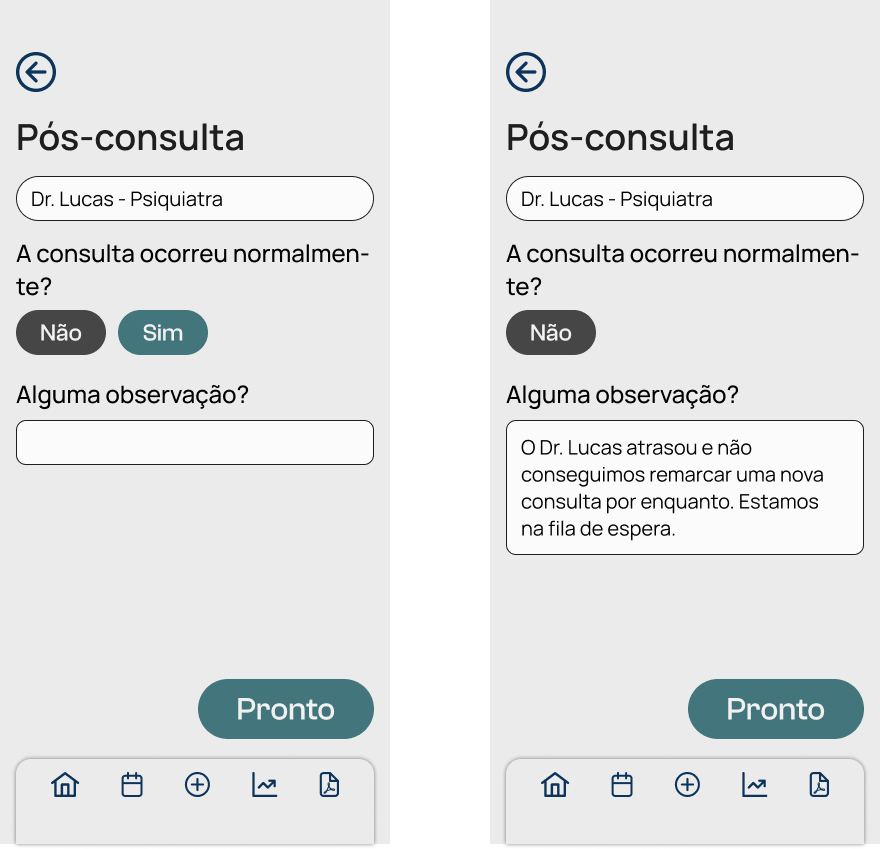
\includegraphics[width=1.0\linewidth]{MyMed - Modelagem/Avaliação Consulta.png}
	\caption{Avaliação de Consulta}
	\label{avaliacao_consulta}
\end{figure}

\begin{figure}
	\centering
	\includegraphics[width=0.6\linewidth]{MyMed - Modelagem/Calendário - Consulta Finalizada-1.png}
	\caption{Calendário - Consulta Finalizada 1}
	\label{calendario_consulta_finalizada_1}
\end{figure}

\begin{figure}
	\centering
	\includegraphics[width=0.6\linewidth]{MyMed - Modelagem/Calendário - Consulta Finalizada.png}
	\caption{Calendário - Consulta Finalizada}
	\label{calendario_consulta_finalizada}
\end{figure}

\begin{figure}
	\centering
	\includegraphics[width=0.6\linewidth]{MyMed - Modelagem/Calendário.png}
	\caption{Calendário}
	\label{calendario}
\end{figure}

\begin{figure}
	\centering
	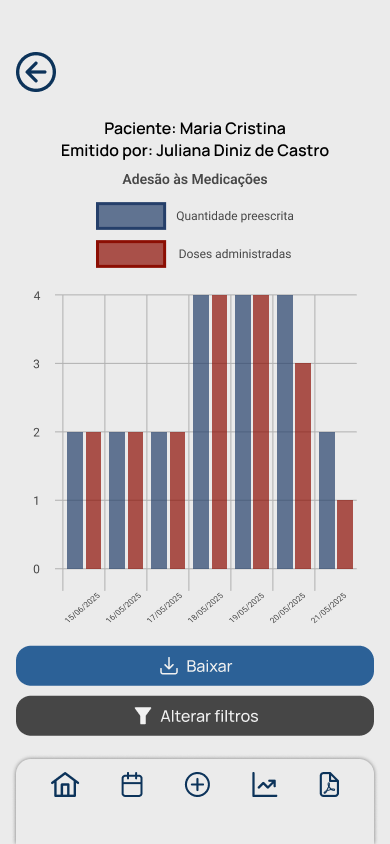
\includegraphics[width=0.6\linewidth]{MyMed - Modelagem/Gráfico - Adesão a Medicações.png}
	\caption{Gráfico - Adesão a Medicações}
	\label{grafico_adesao_medicacoes}
\end{figure}

\begin{figure}
	\centering
	\includegraphics[width=0.6\linewidth]{MyMed - Modelagem/Gráfico - Glicemia.png}
	\caption{Gráfico - Glicemia}
	\label{grafico_glicemia}
\end{figure}

\begin{figure}
	\centering
	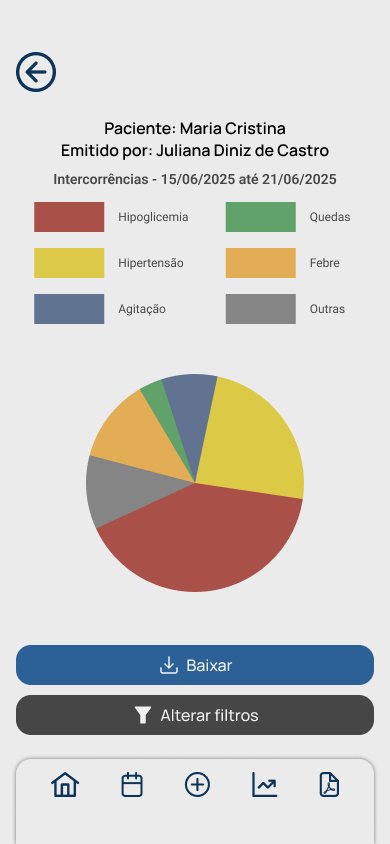
\includegraphics[width=0.6\linewidth]{MyMed - Modelagem/Gráfico - Intercorrências.png}
	\caption{Gráfico - Intercorrências}
	\label{grafico_intercorrencias}
\end{figure}

\begin{figure}
	\centering
	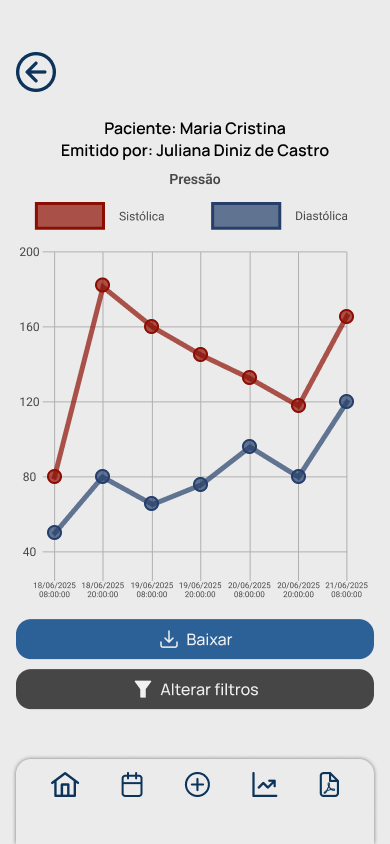
\includegraphics[width=0.6\linewidth]{MyMed - Modelagem/Gráfico - Pressão.png}
	\caption{Gráfico - Pressão}
	\label{grafico_pressao}
\end{figure}

\begin{figure}
	\centering
	\includegraphics[width=0.6\linewidth]{MyMed - Modelagem/Gráficos.png}
	\caption{Gráficos}
	\label{graficos}
\end{figure}

\begin{figure}
	\centering
	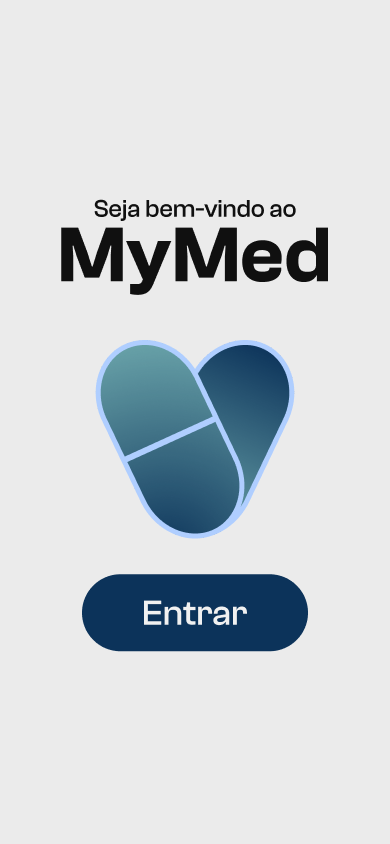
\includegraphics[width=0.6\linewidth]{MyMed - Modelagem/Login.png}
	\caption{Login}
	\label{login}
\end{figure}

\begin{figure}
	\centering
	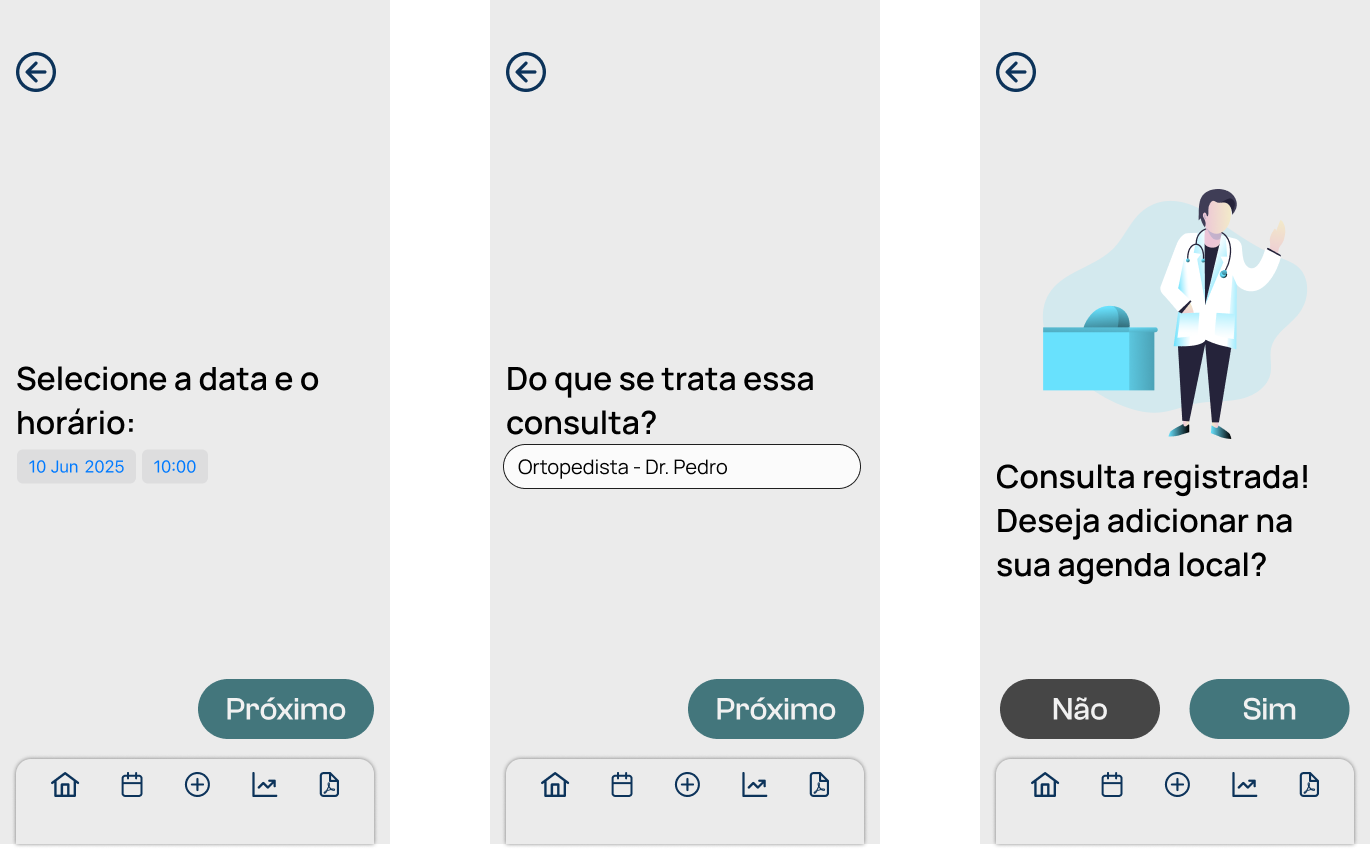
\includegraphics[width=1.0\linewidth]{MyMed - Modelagem/Nova Consulta.png}
	\caption{Nova Consulta}
	\label{nova_consulta}
\end{figure}

\begin{figure}
	\centering
	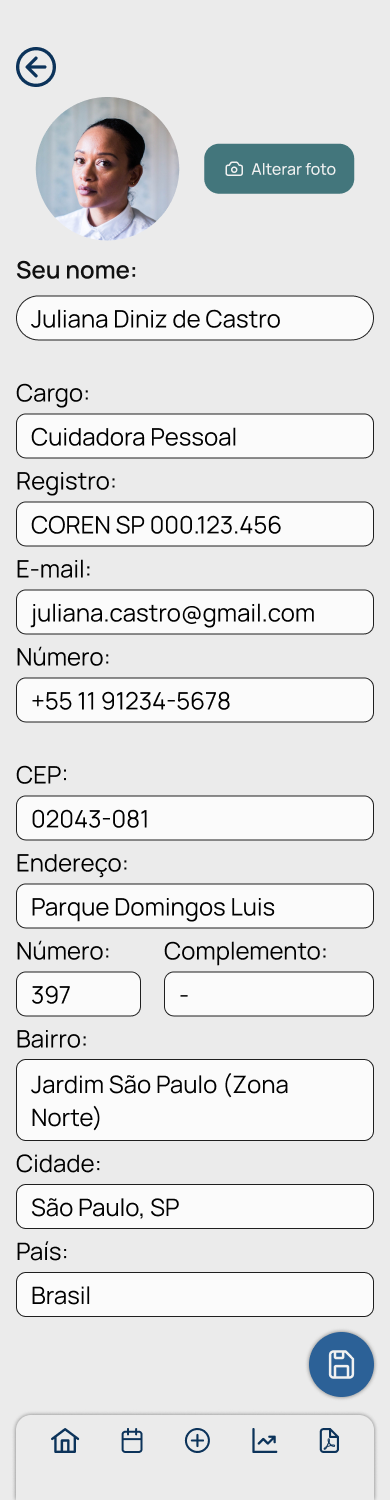
\includegraphics[width=0.4\linewidth]{MyMed - Modelagem/Perfil - Edição.png}
	\caption{Perfil - Edição}
	\label{perfil_edicao}
\end{figure}

\begin{figure}
	\centering
	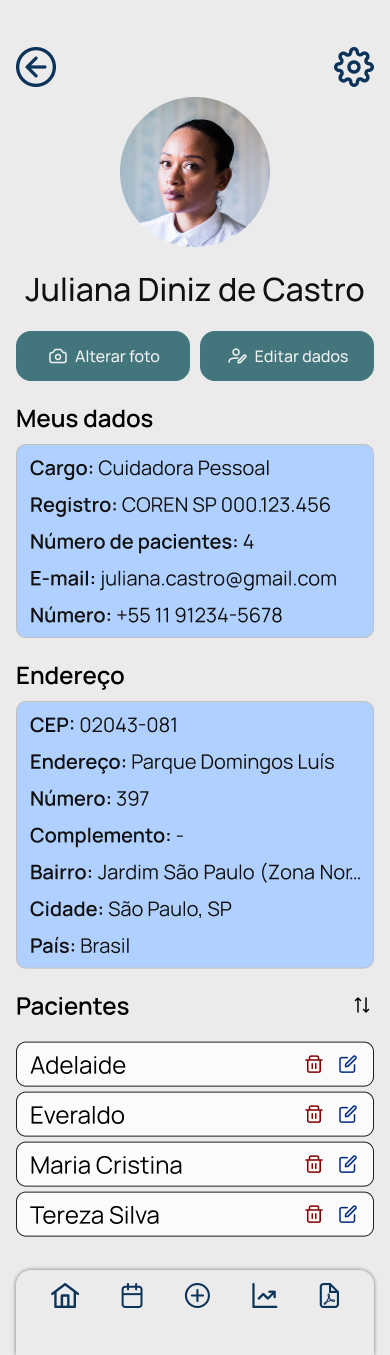
\includegraphics[width=0.4\linewidth]{MyMed - Modelagem/Perfil.png}
	\caption{Perfil}
	\label{perfil}
\end{figure}

\begin{figure}
	\centering
	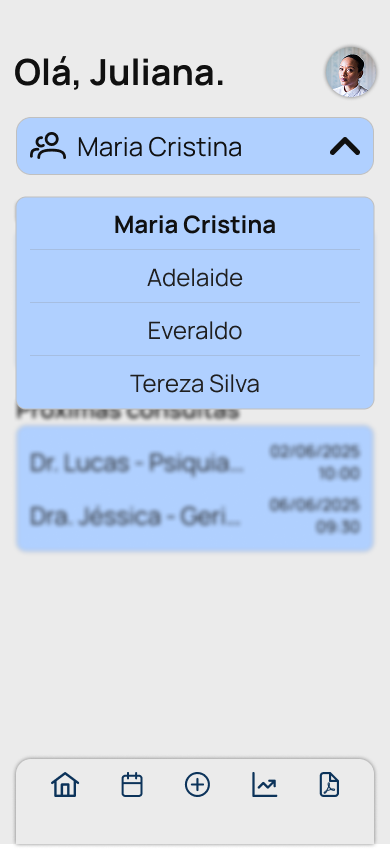
\includegraphics[width=0.6\linewidth]{MyMed - Modelagem/Tela Inicial - Dropdown Nomes.png}
	\caption{Tela Inicial - Dropdown Nomes}
	\label{tela_inicial_dropdown_nomes}
\end{figure}

\begin{figure}
	\centering
	\includegraphics[width=0.6\linewidth]{MyMed - Modelagem/Tela Inicial (Botão +).png}
	\caption{Tela Inicial (Botão +)}
	\label{tela_inicial_botao_mais}
\end{figure}

\begin{figure}
	\centering
	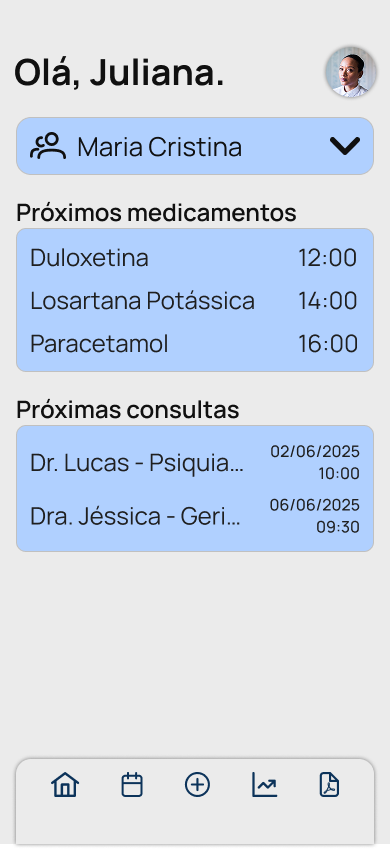
\includegraphics[width=0.6\linewidth]{MyMed - Modelagem/Tela Inicial.png}
	\caption{Tela Inicial}
	\label{tela_inicial}
\end{figure}


\end{apendicesenv}

% % ----------------------------------------------------------
% % Anexos
% % ----------------------------------------------------------
% \cftinserthook{toc}{AAA}
% % ---
% % Inicia os anexos
% % ---
% %\anexos
% \newpage
% \begin{anexosenv}

% % ---
% \chapter{Cras non urna sed feugiat cum sociis natoque penatibus et magnis dis
% parturient montes nascetur ridiculus mus}
% % ---

% Anexos são os documentos não elaborados pelo autor, que servem de fundamentação, comprovação ou ilustração, como mapas, leis, estatutos etc.

% Os apêndices devem aparecer após as referências, e os anexos, após os apêndices.

% \end{anexosenv}

\end{document}
